\documentclass[a4paper,onesided,12pt]{report}
\usepackage{styles/fbe_tez}
\usepackage[utf8]{inputenc} % To use Unicode (e.g. Turkish) characters
\renewcommand{\labelenumi}{(\roman{enumi})}
\usepackage{amsmath, amsthm, amssymb}
% Some extra symbols
\usepackage[bottom]{footmisc}
\usepackage{cite}
\usepackage{graphicx}
\usepackage{longtable}
\graphicspath{{figures/}} % Graphics will be here

\usepackage{multirow}
\usepackage{subfigure}
\usepackage{algorithm}
%\usepackage{algorithmic}
\usepackage{algpseudocode}
%\pagestyle{empty}
%\includeonly{introduction} % To only process the given file


\newtheorem{thm}{Theorem}[chapter]
\newtheorem{prop}[thm]{Proposition}
\newtheorem{lem}[thm]{Lemma}
\newtheorem{cor}[thm]{Corollary}



% COVER PAGE
\title{AIRFLOW ESTIMATION FROM RESPIRATORY SOUNDS}
\turkcebaslik{SOLUNUM SESLERİNDEN SOLUK AKIŞI KESTİRİMİ}
\degree{B.S., Electrical \& Electronics Engineering, Boğaziçi University, 2013}
\author{İlhan Yıldırım}
\program{Electrical \& Electronics Engineering}
\subyear{2018}

% APPROVED BY PAGE
\supervisor{Prof. Yasemin Z. Kahya}
\cosuperi{Assist. Prof. İpek Şen}
%\cosuperii{Title and Name of Cosupervisor II}
\examineri{Prof. Murat Saraçlar}
\examinerii{Assoc. Prof. Rifat Koray Çiftçi}
%\examineriii{}
%\examineriv{}
%\examinerv{}
\dateofapproval{24.5.2018}

\usepackage{etoolbox}
\makeatletter
\patchcmd{\@sect}{\underbar}{\underline}{}{}
\makeatother

\usepackage{tikz}
\usetikzlibrary{shapes, calc, shapes, arrows}
\DeclareMathOperator*{\argmin}{arg\,min}
\begin{document}
	
	\pagenumbering{roman}
	\makemstitle % M.S. thesis
	\makeapprovalpage
	\begin{acknowledgements}
		Acknowledgements come here...
	\end{acknowledgements}
	\begin{abstract}
		One page abstract will come here.  
	\end{abstract}
	\begin{ozet}
		Bir sayfa uzunluğunda özet gelecektir.
	\end{ozet}
	\tableofcontents
	\listoffigures
	\listoftables
	\begin{symbols}
		% The title will be typeset as "LIST OF SYMBOLS".
		%
		% Use a separate \sym command for each symbols definition.
		% First Latin symbols in alphabetical order
		
		\sym{$a_{ij}$}{Description of $a_{ij}$}
		\sym{$\mathbf{A}$}{State transition matrix of a hidden Markov model}
		% Then Greek symbols in alphabetical order
		\sym{}{}
		\sym{$\alpha$}{Blending parameter \textit{or} scale}
		\sym{$\beta_t(i)$}{Backward variable}
		\sym{$\Theta$}{Parameter set}
		\sym{ }{}
		
	\end{symbols}
	
	\begin{abbreviations}
		% Abbreviations in alphabetical order
		\sym{2D}{Two Dimensional}
		\sym{3D}{Three Dimensional}
		\sym{AAM}{Active Appearance Model}
		\sym{ASM}{Active Shape Model}
	\end{abbreviations}
	

\chapter{INTRODUCTION}
\pagenumbering{arabic}
Listening to respiratory sounds to gain information about respiratory diseases is a method which has been applied for at least 2400 years. Since then, different auscultation techniques have been used. The most widely used tool developed for this purpose is called "stethoscope" and it is invented in 1816 by Rene Laënnec \cite{breath-sounds}. Medicine doctors still use this device to diagnose several diseases such as asthma, bronchitis etc. \par

In recent decades, engineers started to work on respiratory sounds and they produced electronic stethoscopes. These electronic stethoscopes have some
advantages over the traditional ones. First of all, the frequency band
is not limited \cite{advances-beyond-stet} by the mechanic structure of stethoscope and the sounds can be recorded for reuse. Another advantage is that the respiratory sound recordings made analyzing the sound with the help of computers possible. \par
 
In recent years, together with developing classification techniques, there has been a great effort in automatic classification of respiratory sounds as healthy or sick \cite{ipek-svm-gmm}. Some of these methods are dependent not only on sounds but also on the airflow information \cite{lung-subphase}. Airflow is usually recorded by a tool which is called pneumotachograph. This tool is not useful in case of subject who have some disabilities.

Main motivation of this thesis is to estimate the airflow and respiratory phases from the respiratory sounds recorded at chest wall without using pneumotachograph to enable airflow measurements to be easier and a development of single handheld electronic stethoscope whose recording will be enough for automatic diagnose. 

Before giving the preview of the work has been done over this thesis, we may give a brief review of the literature about the relation between flow, phase and respiratory sounds.

\textit{Lessard and Wong} \cite{corr-cons-flow-spectrum} reported that the relation between the spectral parameters which are mean frequency, frequency of maximum power and the highest frequency at which the power in the spectrum is at least 10 percent of maximum power, and flow rate is not linear and spectral parameters saturates as the flow rate goes beyond 0.75 $l/s$. \par
\textit{Yadollahi and Moussavi} \cite{entropy-tracheal} reported that using entropy of bandpass filtered tracheal sounds by using overlapping windows whose durations are 100 milliseconds. They achieved average error of 7.3 \% and 7.4 \% for inspiratory and expiratory phases after calibrating the model which uses the entropy information.\par
\textit{Huq and Moussavi} \cite{saiful-moussavi-log-variance} proposed using log of variance (LV) first to detect onsets. For phase identification, they used 4 parameters calculated over LV curve and the duration of phase. They developed and tested the method for tracheal sounds and it is reported that 95.6\% accuracy was achieved for phase identification after onsets are verified by visual inspection.\par
\textit{Moussavi et al.} \cite{computerised-acoustical-phase} suggested using tracheal sounds for onset detection and the power difference in 150-450 Hz at the "best recording position", where the difference in power for inspiration and expiration is greatest, for phase identification. It is reported that the success rate in phase identification is 100\% after the onsets are found.\par
\textit{Golabbakhsh et al.} \cite{flow-trachea-adaptive} suggested using the average power $(P_{ave})$ of tracheal sounds to estimate the respiratory flow. They have two approaches, first one is expressing the flow as a linear function of log of $P_{ave}$ as in \ref{linear_log_p_ave} and the other one is training an adaptive filter with three taps and whose input is $P_{ave}$ as in \ref{adaptive_p_ave}. 
\begin{align}
	\hat{F} = c_0 + c_1 \log(P_{ave}) \label{linear_log_p_ave}\\
	\hat{F} = \sum_{i=1}^{M}w_iP_{ave} \label{adaptive_p_ave}
\end{align} \par
\textit{Çiftçi and Kahya} \cite{koray-ieee-embs} modeled the sounds recorded at both trachea and chest as time varying autoregressive (TVAR) processes by using Fourier basis functions and used the first autoregressive (AR) coefficient vector as the estimate of absolute airflow curve. Reported correlations for sounds recorded at trachea and chest wall were 0.9 and about 0.6 (extracted from figure in paper) respectively. \par
Organization of thesis will be explained in following paragraphs. \par
In chapter \ref{chp:exp-setup-data}, the experimental setup and data will be explained. \par 
In chapter \ref{chp:airflow_curve_estimation}, we will describe AR and TVAR processes and the methods to find TVAR coefficients of a signal, the methods we will describe and use are windowing based AR modeling, TVAR modeling with basis functions and Kalman filter. We will also present Short Time Fourier Transform (STFT) and Wiener filter which will be used to unify different estimations. Finally experiments and results will be presented. \par
In chapter \ref{chp:airflow_phase_estimation}, the method for period estimation will be given first. Then neural networks approach and features will be explained. After neural networks, the method which estimates the transition points and then identifies the phases between estimated transition points will be described. Lastly, experiments and results will be documented. \par 
In the conclusion chapter, the last words about this work will be said.
 
\chapter{EXPERIMENTAL SETUP AND DATA}
\label{chp:exp-setup-data}
The data used throuhout this thesis is taken from the database belonging Boğaziçi University Lung Acoustics Laboratory. All sound and airflow samples were recorded with the device developed in this laboratory. (İpek Sen Masters) The recording device has 14 channels. Each channel has the same analog interface, which includes a Sony ECM-44 BPT electret microphone followed by an analog amplifier with gain 100 which has a instrumentation amplifier based design. The amplification unit is followed by a $6^{th}$ order Butterworth low pass filter which have 4000 Hz cut-off and a $8^{th}$ order Bessel high pass filter whose cutoff is 80 Hz. The airflow recordings was done with a Validyne CD379 pneumatachograph. The digitization unit is the National Instrument's DAQCard-6024E which is operating at 9600 Hz and has 12 bit resolution. Each recording has a duration of 15 seconds \cite{ipek-device}.
\paragraph{} There are 23 healthy subjects in this study. The sounds were recorded at 14 different locations on chest wall. Locations of channels are shown in \ref{fig:mic_loc}.
\begin{figure}
	\begin{center}
		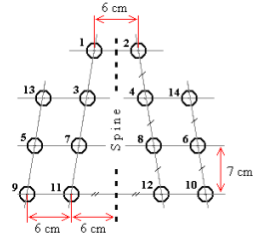
\includegraphics[width=0.4\textwidth]{figures/mic_loc.png}
		\caption{Microphone Locations on the Chest Wall \cite{ipek-phd-2}}
		\label{fig:mic_loc}
	\end{center}
\end{figure} \par
\chapter{AIRFLOW CURVE ESTIMATION}
\label{chp:airflow_curve_estimation}
\section{Autoregressive Models}
Autoregressive modeling is a widely used method in spectral signal analysis. It is also used in respiratory signal analysis and since the respiratory sounds have spectral characteristics changing over time, either we divide the sound into small pieces and assume the small pieces are stationary or we model the respiratory sounds as time varying autoregressive processes. It is reported that when a respiratory sound signal is modeled as TVAR process, the first AR coefficient is highly correlated with the airflow for the sounds recorded at trachea and have less but still correlation for the sounds recorded at chest wall \cite{koray-ieee-embs}. We will test this for the sounds recorded at chest wall and try to find best settings for most correlation in this subsection. We will try to extract the AR coefficients with three methods:
\begin{itemize}
	\item Windowing Based Autoregressive Modeling: Divide the signal into overlapping windows assume each window is independent from others.
	\item Time Varying Autoregressive Modeling with Basis Functions: Assume the AR parameters are combination of sinusoidal signals. 
	\item Time Varying Autoregressive Modeling with Kalman Filter: Assume the AR parameters are changing slowly.
\end{itemize}
\subsection{Univariate Autoregressive Model}
Univariate AR model is a difference equation where the current measurement of the signal is a linear combination of past measured values and a white Gaussian noise. The model is equivalent to a filter with infinite impulse response where the input is white Gaussian noise. The equation of an AR model is given in \eqref{eq_univar_ar}. In this equation $a_{i}$ is the $i^{\text{th}}$ order AR coefficient, $N$ is the order of model and $e$ is the noise term where $\mu_e=0$ and $\sigma_e^2$ is constant \cite{random-signals}. 
\begin{equation}\label{eq_univar_ar}
x(n) = \sum_{i=1}^{N}{a_ix(n-i)} + e(n) 
\end{equation} \par
Before looking at mean, variance, autocorrelation and spectral content of a general AR model, we must set some conditions on $a_{i}$'s to make the model stationary. The stationarity requires the mean, variance and autocorrelation function is constant. If the mean is constant then \eqref{eq_univar_ar_mean} must hold. We know that $\mu_e$ is 0, then either $\sum_{i=1}^{N}{a_i} = 1$ or $\mu_x = 0$ is true. 
\begin{equation}\label{eq_univar_ar_mean}
\mu_x = \sum_{i=1}^{N}{a_i\mu_x} + \mu_e 
\end{equation} \par
We require $E[X(0)] = 0$ for initial conditions for AR processes and it ensures $\mu_x=0$. Then for variance we can write the equations in \eqref{eq_univar_ar_autocorr_1}, \eqref{eq_univar_ar_autocorr_2} and \eqref{eq_univar_ar_autocorr_3}.
\begin{align}
\sigma_{X}^2 = E[X(n)X(n)] - \mu_{X}^2 \label{eq_univar_ar_autocorr_1} \\
\sigma_{X}^2 = \sum_{i=1}^{N}a_iE[X_nX_{n-i}] + E[X_ne_n] - \mu_{X}^2 \label{eq_univar_ar_autocorr_2}\\
\sigma_{X}^2 = \sum_{i=1}^{N}a_iR_{XX}(i) + \sigma_e^2 \label{eq_univar_ar_autocorr_3}
\end{align} \par
We know that autocorrelation coefficients are very important in analysis of an AR model. The AR coefficients can be directly calculated in presence of autocorrelation coefficients.
\begin{align}
	r_{xx}(i) = R_{xx}(i)/R_{xx}(0) \label{eq_univar_ar_corrcoef_1}\\
	r_{xx}(i) = E[x(n)x(n-i)]/R_{xx}(0) \label{eq_univar_ar_corrcoef_2} \\
	r_{xx}(i) = \frac{\sum_{j=1}^{N}{E[a_jx(n-j)x(n-i)]}}{R_{xx}(0)} \label{eq_univar_ar_corrcoef_3}\\
	r_{xx}(i) = \sum_{j=1}^{N}{a_jr_{xx}(i-j)} \label{eq_univar_ar_corrcoef_4}
\end{align} \par
The equation in \eqref{eq_univar_ar_corrcoef_4} is very useful since we can rewrite it as in \eqref{eq_univar_ar_yulewalker}, this equation is called Yule-Walker equation. So, given a signal generated with an AR model, we can find the coefficients of that model by solving the equation in \eqref{eq_univar_ar_yulewalker}. Let's call this equation as $r=Ra$, the the coefficients can easily be found with $a=R^{-1}r$. 
\begin{equation}\label{eq_univar_ar_yulewalker}
\begin{pmatrix}
r_{XX}(1) \\ 
r_{XX}(2) \\ 
\vdots \\ 
r_{XX}(N-1)\\ 
r_{XX}(N) 
\end{pmatrix} =  
\begin{pmatrix}
1 & r_{XX}(1) & ... & r_{XX}(N-2) & r_{XX}(N-1) \\
r_{XX}(1) & 1 & ... & ... & r_{XX}(N-2) \\
\vdots    & \vdots    & \vdots & \vdots & \vdots \\
r_{XX}(N-2) & ... & ... & 1 & r_{XX}(1) \\
r_{XX}(N-1) & r_{XX}(N-2) & ... & r_{XX}(1) & 1
\end{pmatrix} 
\begin{pmatrix} 
a_{1} \\ 
a_{2} \\
\vdots \\
a_{N-1} \\
a_{N} \end{pmatrix}
\end{equation} \par
Although solving the equation \eqref{eq_univar_ar_yulewalker} seems to be very straightforward, it requires exact knowledge on correlation coefficients. However, when we are given a signal with finite length we can just estimate the correlation coefficients, and the error in calculated AR coefficients will depend on the condition number of R matrix. To solve this equation, there are several methods in literature, throughout this thesis we will use Burg's Method to find the AR coefficients, since it is more stable than the others \cite{delft-burg}.
\begin{algorithm}
	\caption{AR Coefficients Estimation With Overlapping Windows}
	\label{Windowed AR}
	\begin{algorithmic}[1]
		\Procedure{WindowedAR}{signal, order, winLen, overlap}
		\State $windowStart \gets 1$; $L \gets {Length(signal)}$;
		\While{$windowStart \leq L-winLen$}
		\State $temp \gets signal(windowStart:(windowStart+windowLength))$;
		\State $AR(:,i) \gets EstimateAR(temp, N)$;
		\State $windowStart \gets windowStart + windowLength$;
		\EndWhile
		\State \textbf{return} $AR$;
		\EndProcedure
	\end{algorithmic}
\end{algorithm}\\

\subsection{Time Varying Autoregressive Model}
While univariate autoregressive model is very useful for many signals, the method doesn't use the continuity of the signal and treats each segment independently. Assuming the coefficients at different time instants are correlated with each other and building some structured models is another method which is widely applied for nonstationary signals. TVAR modeling were applied to respiratory signals and satisfactory results have been obtained in many papers. The equation describing a TVAR process is given in \eqref{eq_tvar}. 
\begin{equation}\label{eq_tvar}
x(n) = \sum_{i=1}^{N}{a_i(n)x(n-i)} + e(n) 
\end{equation} \par
We will use two methods for solving this equation for $a_i$s. One of them is modeling $a_i$s as combination of sinusoids, the other one is modeling $a_i$s as slowly changing parameters.

\subsubsection{TVAR Coefficients Estimation With Fourier Basis Functions}
In this method, the AR coefficients are assumed to be combination of sinusoidal functions. Then equations in \eqref{eq_tvar_basis} and \eqref{eq_tvar_basis_2} can be written.
\begin{align}
x(n) = \sum_{i=1}^{N}{x(n-i)\sum_{j=1}^{M}{c_{ij}u_j(n-i)}} + e(n) 
\label{eq_tvar_basis}\\
a_{i}(n) = \sum_{j=1}^{M}{c_{ij}u_j(n-i)}
\label{eq_tvar_basis_2}
\end{align} \par
Equation \eqref{eq_tvar_basis} can be rewritten in vector form as in \eqref{eq_tvar_vector} where $X_{i}$ is the diagonal matrix with the diagonal elements are adjacent elements of $x$ starting from $i$, $U$ is the matrix whose columns are basis vectors, and the $c_{i}$'s are the unknown parameters in this equation.
\begin{equation} \label{eq_tvar_vector}
	x = \sum_{i=1}^{N}X_{i}Uc_{i} + e
\end{equation} \par
Let $Y_{i} = X_{i}U$, the equation can be written in matrix form as in 
\begin{equation}\label{matrix_form}
x = 
\begin{pmatrix}
Y_{1} | Y_{2}  
\hdots Y_{N}
\end{pmatrix} 
\begin{pmatrix}
c_{1} \\
c_{2} \\
\vdots \\
c_{M}
\end{pmatrix}
+ e
\end{equation} \par
The equation in \eqref{matrix_form} describes an overdetermined set of equations, we will use least squares approach to solve this. After finding {$\textbf{c}$} vector, which has $NxM$ elements, calculating $a_{i}(n)$, TVAR coefficients, will be straightforward.
\begin{equation}
	\textbf{c} = (Y^{T}Y)^{-1}Y^{T}x
\end{equation} \par
We will try to find the optimum values for AR order, number of basis vectors, and the range of frequencies spanned by basis vectors to get the best correlation.
\begin{algorithm}
	\caption{TVAR Coefficients Estimation With Fourier Basis Functions}
	\label{Basis TVAR}
	\begin{algorithmic}[1]
		\Procedure{TVARFourierBasis}{signal, order, freqRange, numBasis}
		\State $\delta_f=freqRange/numBasis$;
		\For{i=1:numBasis}
		\State $U(:,2*i-1)$ $=$ $sin(i*\delta_{f})$;
		\State $U(:,2*i)$ $=$ $cos(i*\delta_{f})$;
		\EndFor
		\State $Generate$ $Y$: $Project$ $signal$ $onto$ $U$;
		\State $c$ = $(Y^{T}Y)^{-1}Y^{T}x$
		\For{i=1:N}
			\State $AR(:,i)$ $=$ $U$$c_{i}$;
		\EndFor
		\State \textbf{return} $AR$;
		\EndProcedure
	\end{algorithmic}
\end{algorithm}\\
\subsubsection{TVAR Coefficients Estimation With Kalman Filter}
Kalman filter is a very old but still popular algorithm in field of information processing. It is the minimum mean square estimator for the state of linear dynamical systems \cite{kalman-neural}. It is used everywhere from tracking applications to computer games. \par
Before explaining how Kalman filter works, we must first give the required equations to describe the model where it is applied. Kalman filter is invented to work on dynamic systems where we can record the noisy observations of transformations of the process in interest. So we may give two equations, for both measurement \eqref{Kalman measurement} and process \eqref{Kalman process} model \cite{kalman-seismic}.
\begin{align}
	y_n = H_nx_{n} + v_n \label{Kalman measurement}	\\
	x_n = F_n x_{n-1} + B_n u_n + w_n \label{Kalman process}	
\end{align} \par
In \eqref{Kalman process} $x$ is the state vector, $u$ is control input to the system, $B$ is the control matrix, $F$ is the state transition matrix and $w$ is process noise. In \eqref{Kalman measurement} the $H$ is the transform matrix and $v$ is the measurement noise. When a model desribed in \eqref{Kalman measurement} and \eqref{Kalman process} is present, we can observe $y$ and we are after estimatin $x$, we can apply Kalman filter. When the process and measurement noises are Gaussian then Kalman is the optimal estimator. \par
In our problem, there is not any control input to system and equations convert to \eqref{Kalman measurement respiratory} and \eqref{Kalman process respiratory}. In these equations $y$ is the recorded sound amplitude, $x$ is the AR coefficients, $H$ is equal to raw vector containing previous $N$ values of $y$ where $N$ is the AR order.
\begin{align}
	y_n = H_nx_{n} + v_n \label{Kalman measurement respiratory}	\\
	x_n = F_n x_{n-1} + w_n \label{Kalman process respiratory}	
\end{align} \par
Kalman filter includes two stages, prediction and measurement update. The prediction equations are given in \eqref{Kalman prediction 1} and \eqref{Kalman prediction 2}. The measurement update equations are given in \eqref{Kalman measurement update 1}, \eqref{Kalman measurement update 2} and \eqref{Kalman measurement update 3}. In these equations $\hat{x}_{n|m} = E[x_{n}|y_{1:m}]$ and $P_{n|m} = E[(x_n-\hat{x}_{n|m})(x_n-\hat{x}_{n|m})^T|y_{1:m}]$. \par
Prediction:
\begin{align}
	\hat{{x}}_{n|n-1} = F\hat{{x}}_{n-1|n-1}\label{Kalman prediction 1}	\\
	P_{n|n-1} = FP_{n-1|n-1}F^T + \sigma_{w}^{2} \label{Kalman prediction 2}
\end{align}  \par
Measurement Update:
\begin{align}
	K_n = P_{n|n-1}H(H_n^TP_{n|n-1}H_n + \sigma_{v}^{2})^{-1} \label{Kalman measurement update 1} \\
	\hat{x}_{n|n} = \hat{x}_{n|n-1} + K_n(y_n - H_n^T\hat{x}_{n|n-1}) \label{Kalman measurement update 2} \\
	P_{n|n} = (I-K_nH_n^T)P_{n|n-1} \label{Kalman measurement update 3}
\end{align} \par
In the equations above, the filter uses only measurement values before $N$ to estimate a value of $x_N$. In order to add the information from complete signal, the estimations can be smoothed with Rauch-Tung-Striebel backward recursions given in \eqref{Kalman backward 1}, \eqref{Kalman backward 2} and \eqref{Kalman backward 3}.
\begin{align}
J_n = P_{n|n}F^TP_{n+1|n}^{-1}  \label{Kalman backward 1} \\
\hat{x}_{n|N} = \hat{x}_{n|n} + J_n(x_{n+1|N} - x_{n+1|n}) \label{Kalman backward 2} \\
P_{n|N} = P_{n|n} + J_n(P_{n+1|N} - P_{n+1|n})J_{n}^T \label{Kalman backward 3}
\end{align}  \par
There process noise, state transition matrix and measurement noise are not being updated, and we must tune them. The tuning process and results will be given in Experiments \& Results section.

\section{Time Frequency Analysis}
Short Time Fourier Trasnform is a technique which is widely used and very useful for analysis of signals with a time varying spectral characteristics. STFT is used for analysis of respiratory signals since they have a nonstationary nature. 
\begin{equation}
X_m(f) = \sum_{n=-\infty}^{\infty}x(n)w(n-mR)e^{-j2\pi fn}
\label{STFT}
\end{equation} \par
STFT is defined in \eqref{STFT}. It can be seen as a sliding Fourier Transform (FT) \cite{stft-first}. In this equation, $R$ is hop size and $w$ is the window function which zero outside of a predefined range and is used to pick the part of signal which will be input of FT and smooth the signal to make it stationary. The window is an important parameter for STFT, it is the effective parameter to adjust time-frequency resolution. First of all, the window length must be so small that it must ensure that the selected portion is stationary. There is also a trade-off between resolution in time and resolution in frequency, this trade-off is also controlled with window length. As the  window length increases the frequency resolution increases and the time resolution decreases. So, for wideband signals one can use smaller window lengths whereas for narrowband signals greater window lengths may be used. \par
The output of STFT operation is a two dimensional complex matrix, which describes the magnitude and phase of frequency band component. For most of the time and for respiratory sounds too, we need the magnitude information and we convert the complex matrix to a real matrix which will give information about energy directly. The resulting matrix is usually visualized by a heatmap as in \ref{fig:sound_flow_specgram}.
\begin{figure}
	\begin{center}
		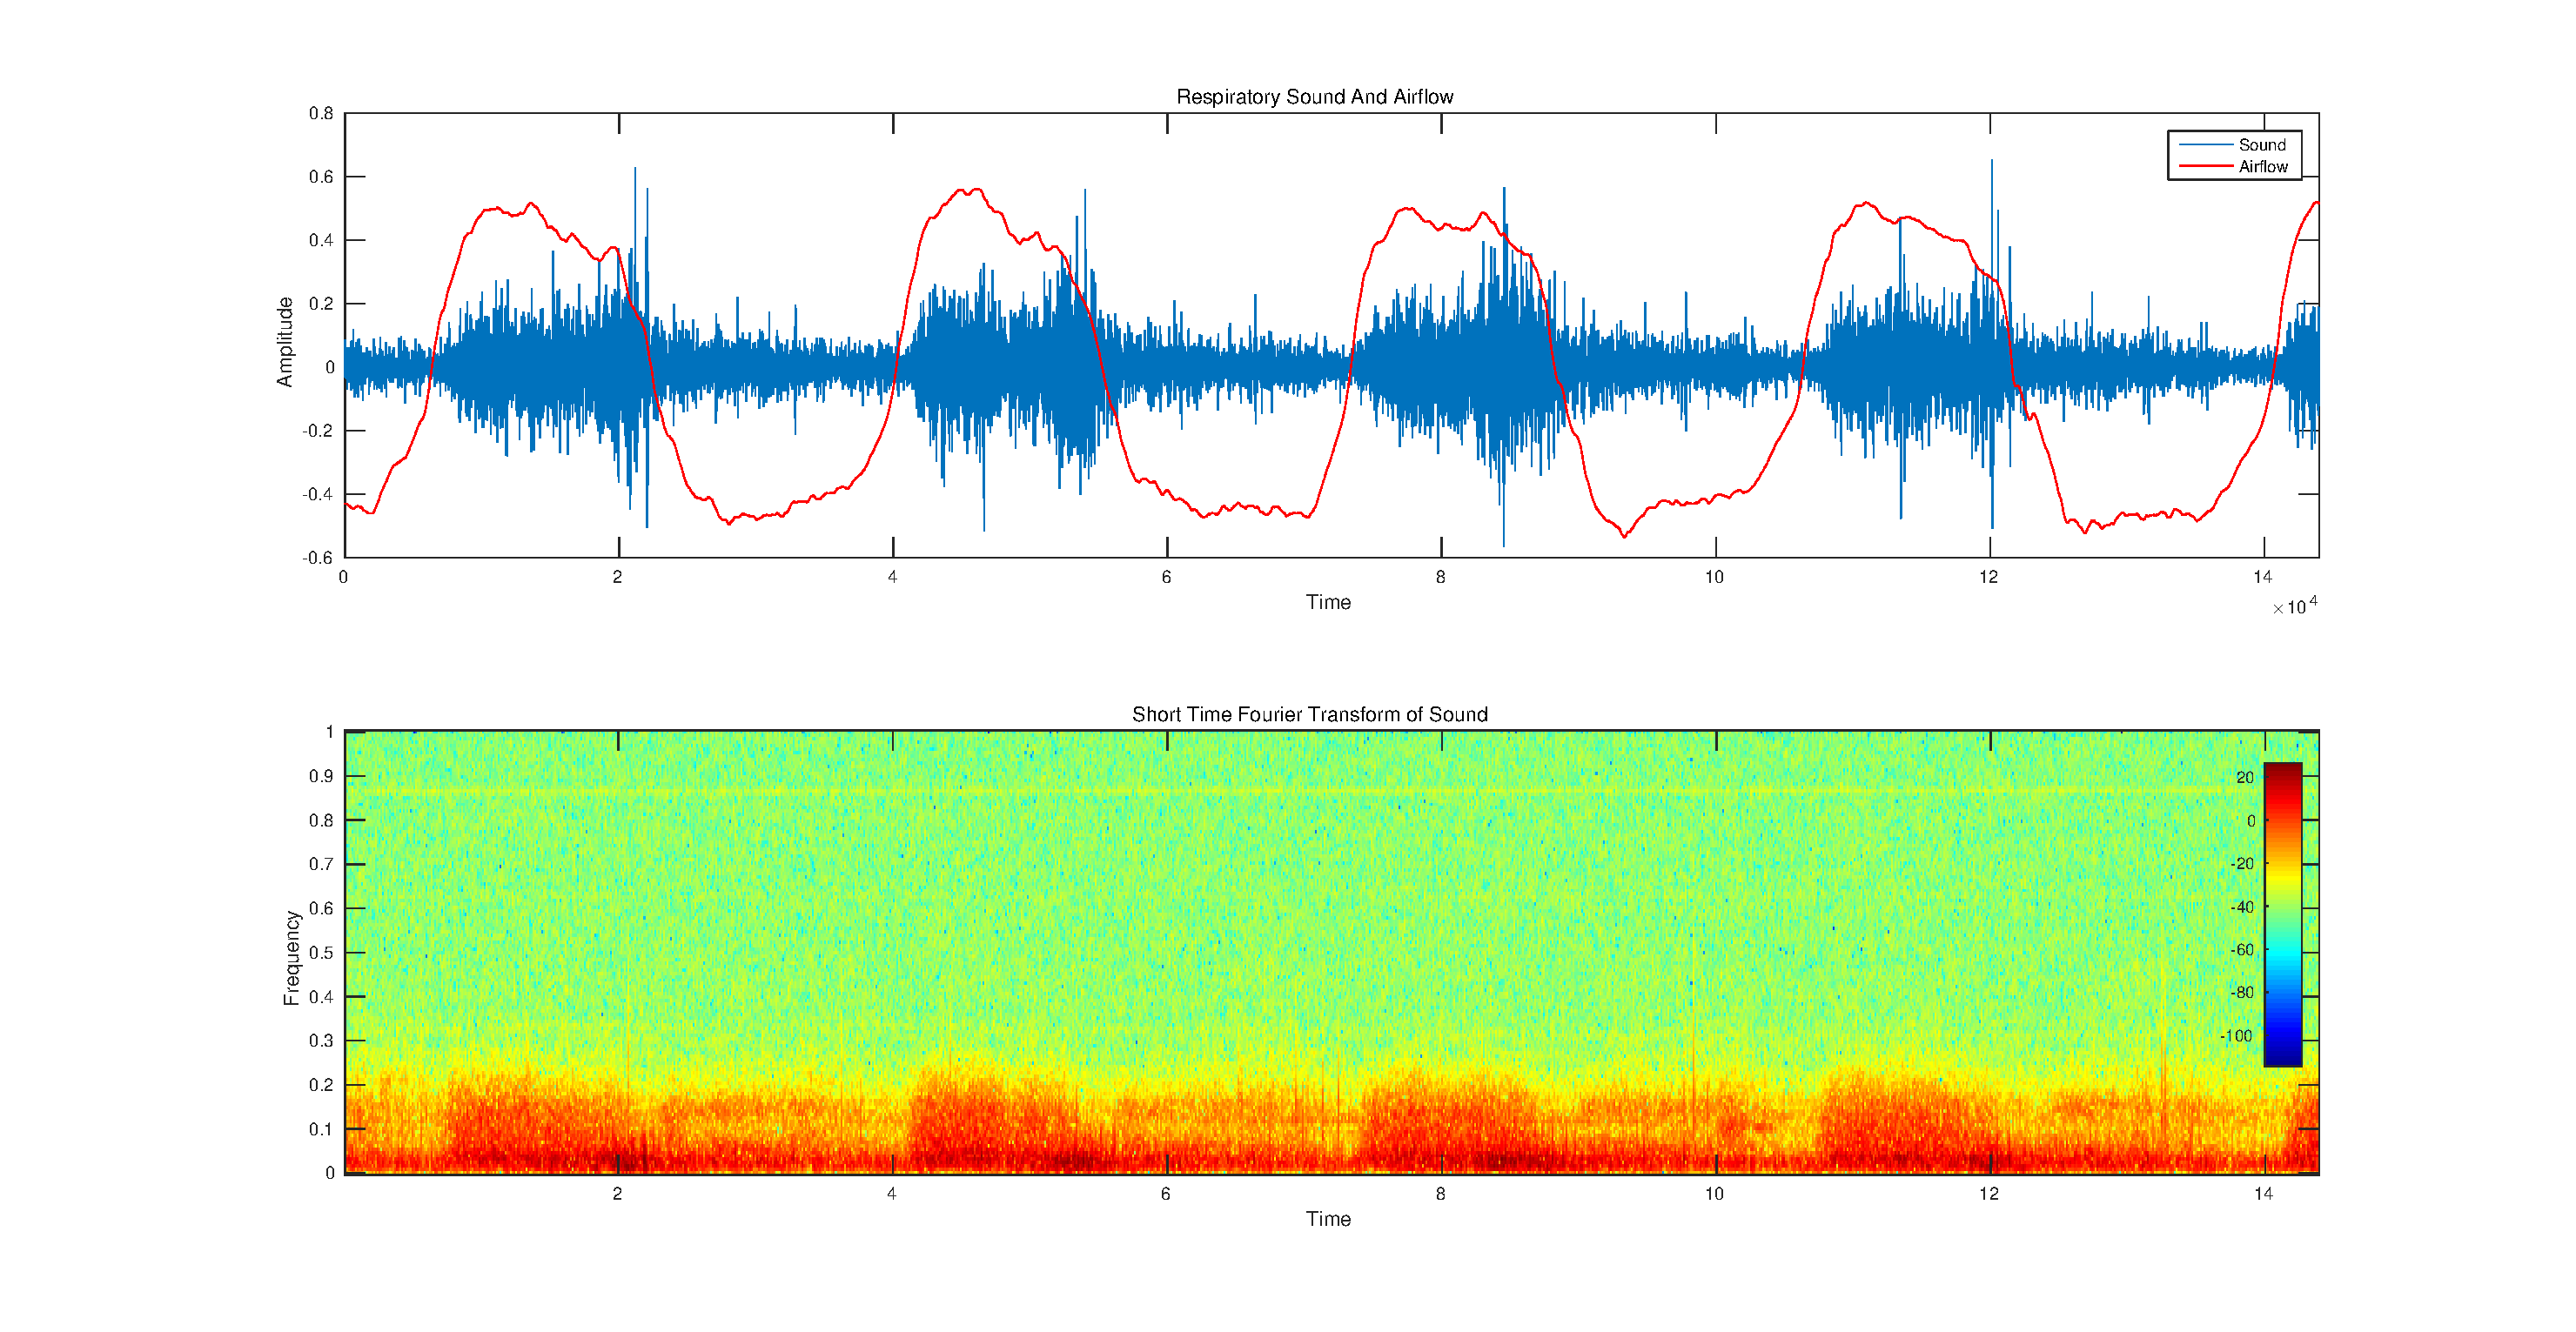
\includegraphics[width=\textwidth]{figures/sound_flow_specgram.eps}
		\caption{A respiratory sound, corresponding airflow and STFT magnitude plot}
		\label{fig:sound_flow_specgram}
	\end{center}
\end{figure} \par
When we look at figure \ref{fig:sound_flow_specgram}, respiratory sound, magnitude plot of its STFT and corresponding airflow we can see a trend seems related to airflow in evolution of some horizontal lines. They correspond to the energy at a frequency band over the time. We will run experiments to test the correlation between the evolution of energy at each frequency band with the airflow. We will tune STFT by tweaking the window type, window length and number of FFT bins in Experiment \& Results. 


\section{Unifying Estimations}
When we have an estimation problem with desired output $d$ and
observations in $x$ vector if each observation in $x$ and $d$ are
jointly wide sense stationary (wss) the optimum estimator for mean
square error (MSE) is the Wiener filter \cite{adaptive-filter-theory}. We can write down the
equations and derive the optimum filter. The estimation equation is
given in \eqref{scalarestimation}, $\hat{d}$ is the estimation in this
equation. Estimation error is given in \eqref{estimationerror} and the
error measure we are interested in is given in
\eqref{errorsquaredopen}
\begin{align}
\hat{d} = \sum_{i=1}^{N}w_ix_i = \bold{w^Tx} \label{scalarestimation} \\
e = d - \hat{d} = d - \bold{w^Tx} \label{estimationerror} \\
E[e^2] = E[|d - \hat{d}|^2] \label{errorsquared} \\
E[e^2] = E[d^2 - 2d\bold{x^T w} + \bold{w^T x x^T w}]
\label{errorsquaredopen}
\end{align} \par
In order to minimize the error we can differentiate with respect to
$\bold{w}$ and find the value where derivative is zero. For error to
be at its minimum the expectation in \eqref{derivative_error} must be
zero, this requires $\bold{x}$ and $e$ to be uncorrelated.
\begin{align}
\frac{\partial E[e^2]}{\partial \boldsymbol{w}} =
2E[e\frac{\partial e}{\partial \boldsymbol{w}}] = -2E[e x_i]
\label{derivative_error}
\end{align} \par
If we rewrite error as difference between $d_n$ and
$\bold{w_{opt}^Tx}$, then we can state the equations in
\eqref{error_observation} and \eqref{error_observation_2}.
\begin{align}
E[(d_n - \bold{w_{opt}^Tx})\bold{x}] = 0 \label{error_observation}\\
E[\bold{xx^T}]\bold{w_{opt}} = E[\bold{x}d_n] \label{error_observation_2}
\end{align} \par
The first expectation in \eqref{error_observation_2} is autocovariance
matrix of $\bold{x}$ and the second expectation is crosscovariance
between $x$ and $d$. The filter $w_{opt}$ is the called as Wiener
filter. \par
In previous sections we end up with vectors which are estimations of
airflow. We will use a weighted sum of these estimations as our
observations and weights will be decided by using this Wiener filter
approach.


\section{Experiments \& Results}
In this section, the experiments to reach the best tuning parameters and the results will be given for the methods explained in this chapter.
\subsection{Univariate Autoregressive Model}
There are 4 parameters to be optimized in univariate autoregressive modeling method. These parameters are the coefficient degree, AR order, window length and overlap.  \par
Firstly, we will try to answer the question about which AR order and which coefficient order is best. For this purpose, experiments will be done for AR orders from 1 to 15 with three different window length 500, and 50\% overlap. 
\begin{figure}
	\begin{center}
		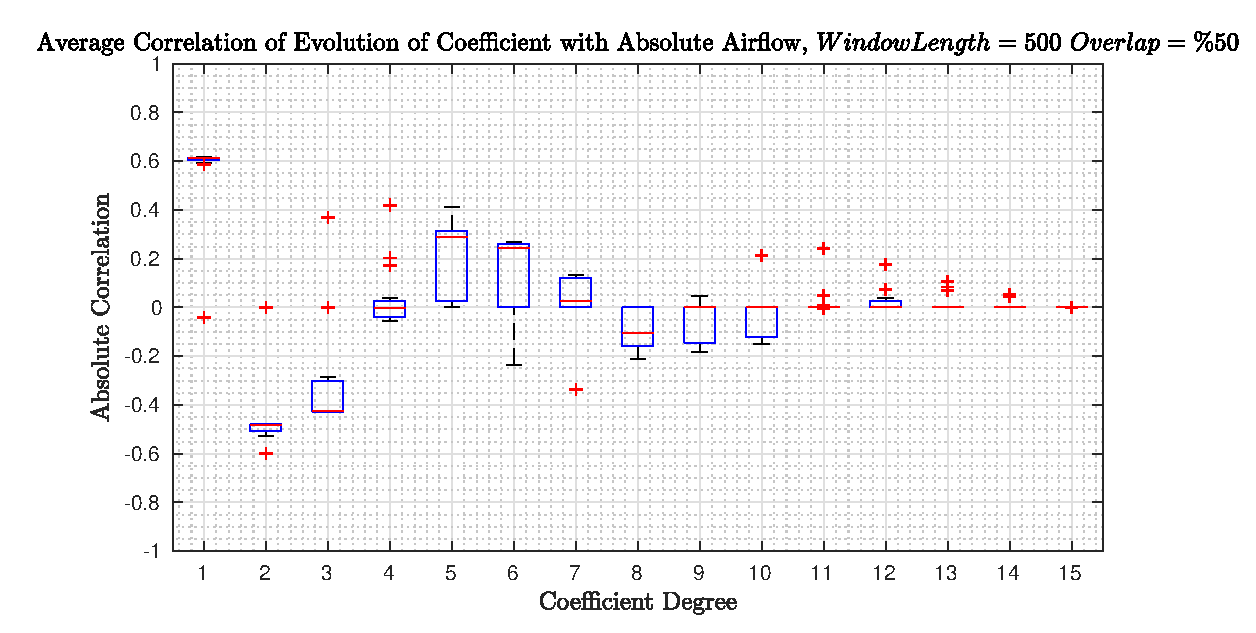
\includegraphics[width=\textwidth]{figures/corr_abs_coeff_for_degree_selection.eps}
		\caption{Boxplot for correlation coefficient of AR coefficient evolution with absolute value of airflow for different coefficient orders}
		\label{fig:absolute_airflow_window_coef}
	\end{center}
\end{figure}
\begin{figure}
	\begin{center}
		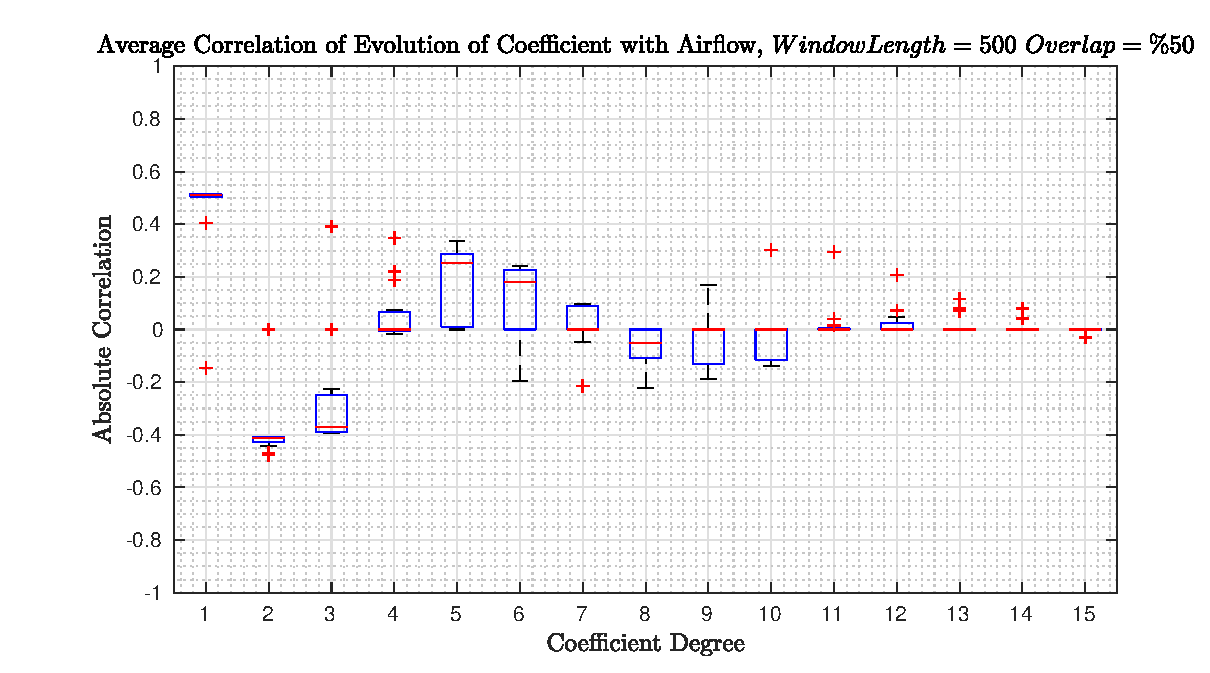
\includegraphics[width=\textwidth]{figures/corr_normal_coeff_for_degree_selection.eps}
		\caption{Boxplot for correlation coefficient of AR coefficient evolution with airflow for different coefficient orders}
		\label{fig:normal_airflow_window_coef}
	\end{center}
\end{figure}
\begin{figure}
	\begin{center}
		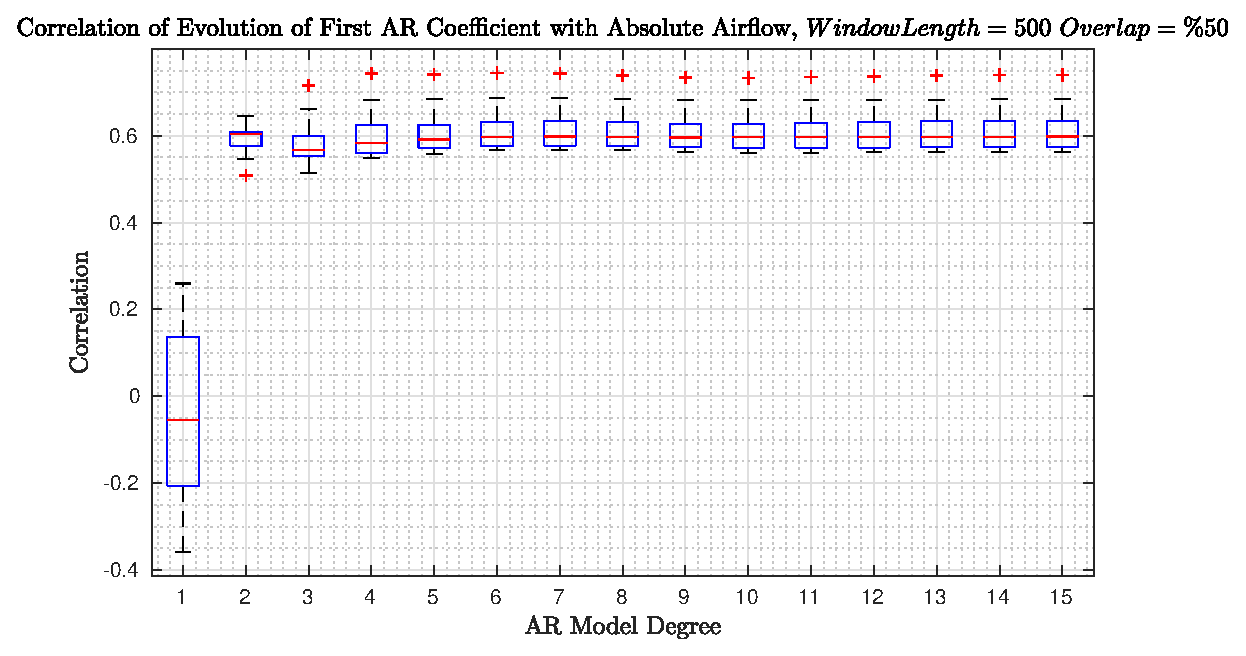
\includegraphics[width=\textwidth]{figures/corr_abs_for_ar_model_degree_selection.eps}
		\caption{Boxplot for correlation coefficient of AR coefficient evolution with airflow for different AR model orders}
		\label{fig:abs_airflow_window_ar_model}
	\end{center}
\end{figure}
\begin{figure}
	\begin{center}
		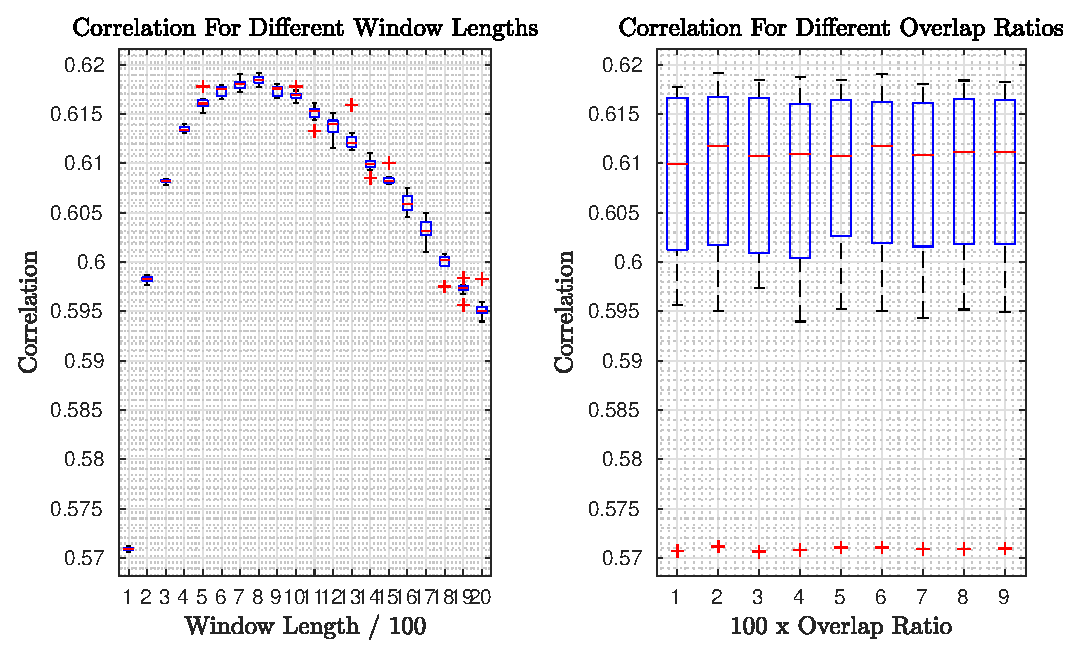
\includegraphics[width=\textwidth]{figures/corr_abs_for_window_length_selection.eps}
		\caption{Boxplot for correlation coefficient of first AR coefficient evolution with absolute airflow for different window lengths and overlap ratios}
		\label{fig:abs_airflow_window_ar_model_window_overlap}
	\end{center}
\end{figure}\par
The inference from figures  is that the correlation is decreasing with increasing coefficient order and the correlation with absolute value of flow is significantly greater. We will continue our analysis with absolute value of airflow for AR estimators. Now we will continue the analysis to find the best model order. For this, we run experiments with window length 500 and an overlap of \%50 with model orders from 1 to 15. The results are shown in figure \ref{fig:abs_airflow_window_ar_model}. As can be seen from figure, there isn't any significant difference after sixth order AR model, so we chose 6 as our model order. After selecting model order, the window length and overlap ratio are left to be decided on. In order to select them we run experiments with window lengths from 100 to 2000 with a seperation of 100 and overlap ratios from 10\% to 90\% with a separation of 10\%. The results for different window lengths and overlap ratios are summarized in figure \ref{fig:abs_airflow_window_ar_model_window_overlap}, according to the results best window length is 800 and difference in overlap ratio doesn't generate any difference in the correlation. We decided to use 90\% overlap to increase the resolution. \par
The resulting decision for univariate autoregressive solution with overlapping windows is 6, 800, 90\% for model order, window length and overlap ratio respectively. 
\subsection{Time Varying Autoregressive Model with Basis Functions}
The parameters for this method are model order, number of basis functions and the frequency difference in adjacent basis functions. \par 
First, we run experiments to determine the best model order and for this purpose run experiments with model orders from 1 to 15 where the number of basis functions are 201 (100 sines, 100 cosines and a constant) and the separation in frequency is 0.04 $Hz$. Experiment results are given in figure \ref{fig:abs_airflow_tvar_model_order}. Most correlation is achieved with the model order of 6 again. \par
After deciding on model order, we need to decide on number of basis functions and frequency separation of basis functions. Before doing this, we run experiments to determine the frequency coverage for best correlation and run experiments with separation of 0.025 $Hz$ and different number of basis frequencies from 50 to 300 with steps of 50. The result is given in figure \ref{fig:abs_airflow_tvar_freq_range}. According to test results 5 $Hz$ is enough to cover for best results.
\begin{figure}
	\begin{center}
		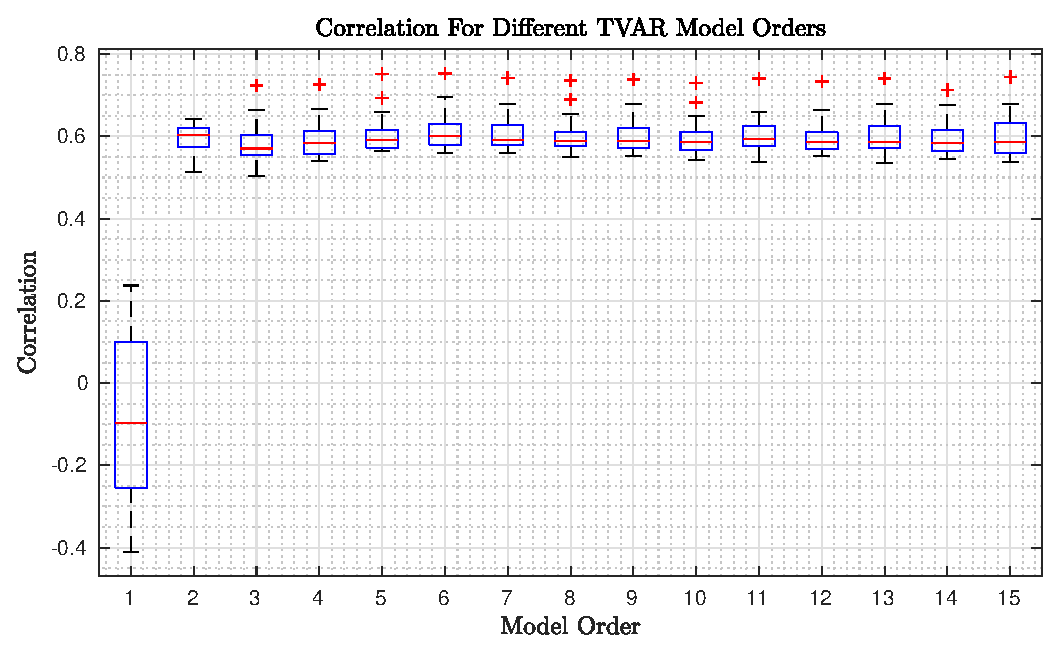
\includegraphics[width=\textwidth]{figures/corr_abs_for_tvar_ar_order_selection.eps}
		\caption{Boxplot for correlation coefficient of first AR coefficient evolution with absolute airflow for different TVAR model orders}
		\label{fig:abs_airflow_tvar_model_order}
	\end{center}
\end{figure}
\begin{figure}
	\begin{center}
		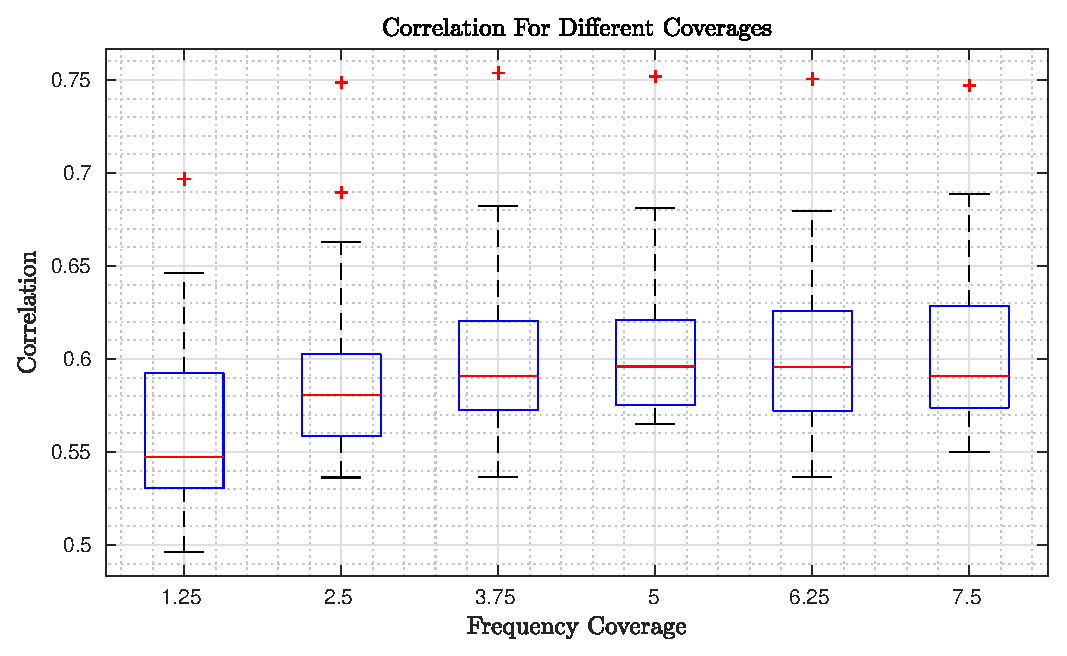
\includegraphics[width=\textwidth]{figures/corr_abs_for_tvar_frange_selection.eps}
		\caption{Boxplot for correlation coefficient of first AR coefficient evolution with absolute airflow for different frequency coverage}
		\label{fig:abs_airflow_tvar_freq_range}
	\end{center}
\end{figure}
Finally we run simulations to decide both the number of basis frequencies and frequency separation and for each tuning we covered the frequency range from 0 to 5 $Hz$. The results are given in figure \ref{fig:abs_airflow_tvar_numbasis_selection}, it shows that it doesn't make significant change to choose number of basis functions as 200 or 400. We chose it to be 250 for minimum standard deviation. \par 
To summarize, 6, 250, 0.02 is chosen for model order, number of basis frequencies and frequency separation respectively.
\begin{figure}
	\begin{center}
		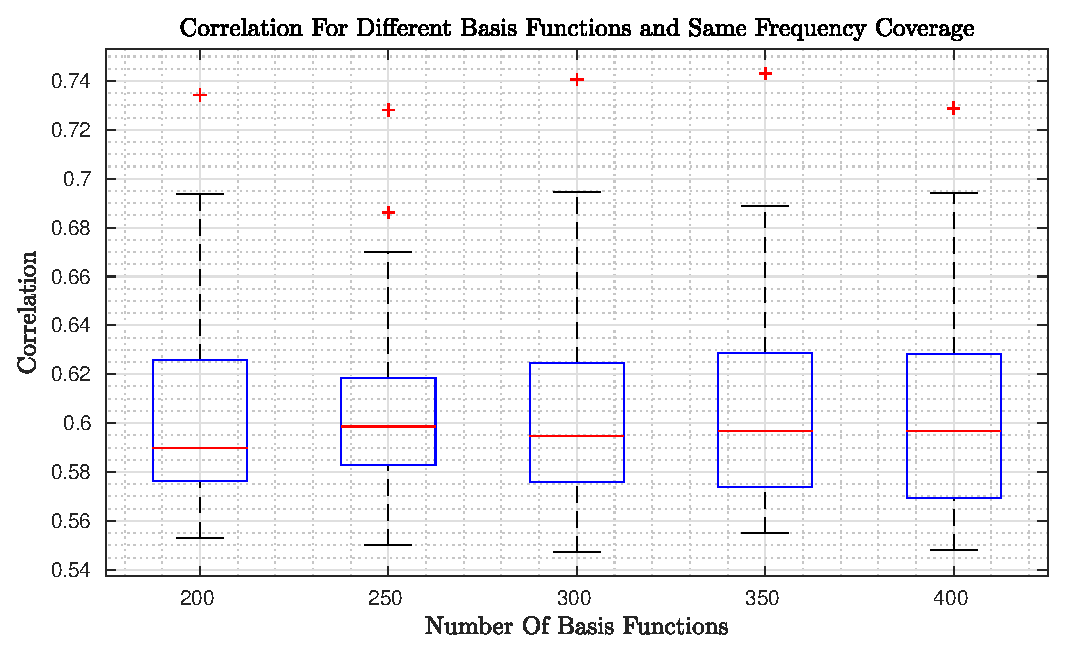
\includegraphics[width=\textwidth]{figures/corr_abs_for_tvar_numbasis_selection.eps}
		\caption{Boxplot for correlation coefficient of first AR coefficient evolution with absolute airflow for number of basis functions}
		\label{fig:abs_airflow_tvar_numbasis_selection}
	\end{center}
\end{figure} \par 

\subsection{Time Varying Autoregressive Model with Kalman Filter}
For this method, we used the noise estimated by windowing based AR modeling as the measurement noise variance, and look for the best noise variance for process noise. We run simulations where the state uncertainity goes from 0.0002 to 0.004 with steps of 0.0002. The results are given in \ref{fig:abs_airflow_kalman_noise_selection}. We chose 0.004 as our process variance.

\begin{figure}
	\begin{center}
		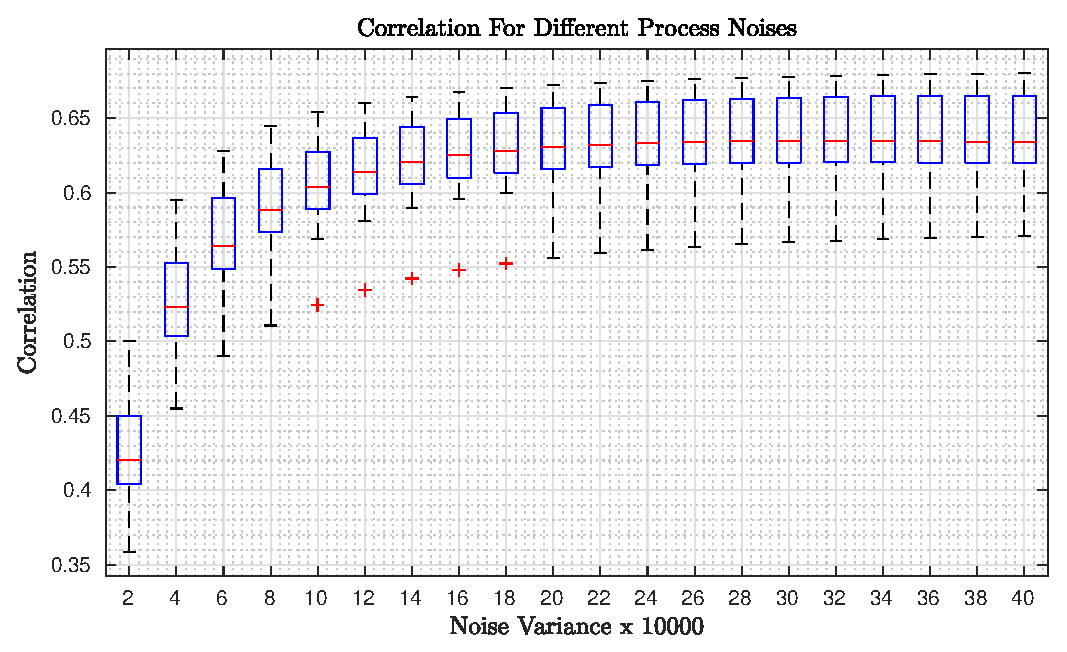
\includegraphics[width=\textwidth]{figures/corr_abs_for_kalman_noise_selection.eps}
		\caption{Boxplot for correlation coefficient of first AR coefficient evolution with absolute airflow for different process noise variances}
		\label{fig:abs_airflow_kalman_noise_selection}
	\end{center}
\end{figure}

\subsection{Short Time Fourier Transform}
\begin{figure}[h!]
	\begin{center}
		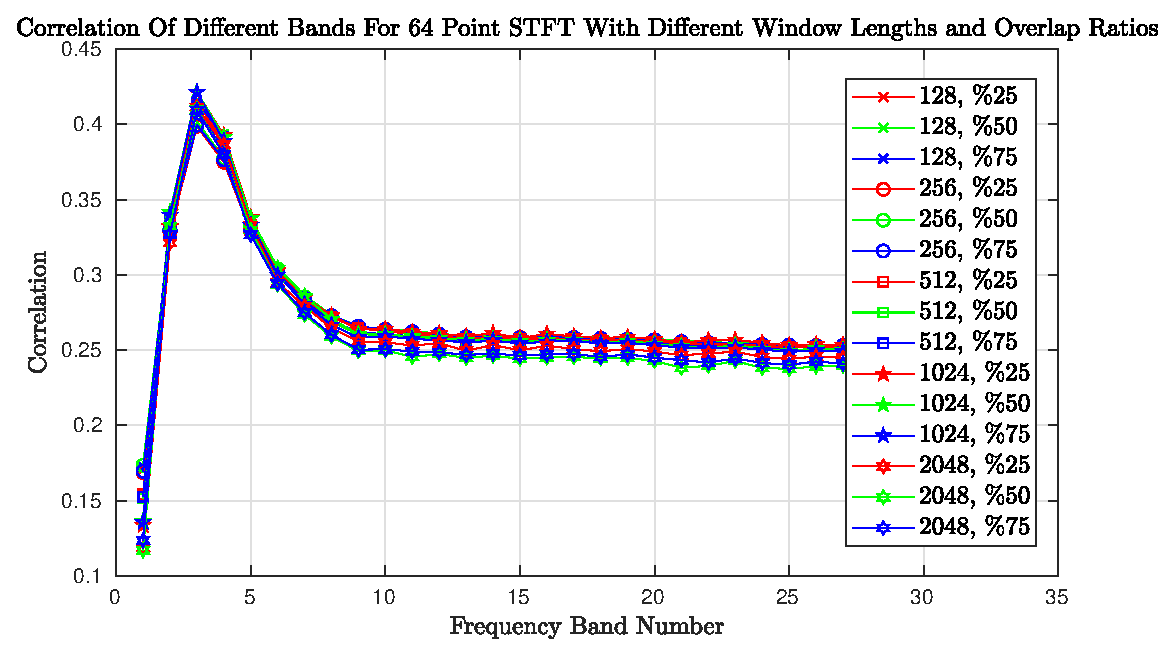
\includegraphics[width=\textwidth]{figures/corr_normal_for_stft_64.eps}
		\caption{Mean of correlations for each band for STFT method with 64 fft bins, window lengths and overlap ratios}
		\label{fig:airflow_stft_64}
	\end{center}
\end{figure}
\begin{figure}[h!]
	\begin{center}
		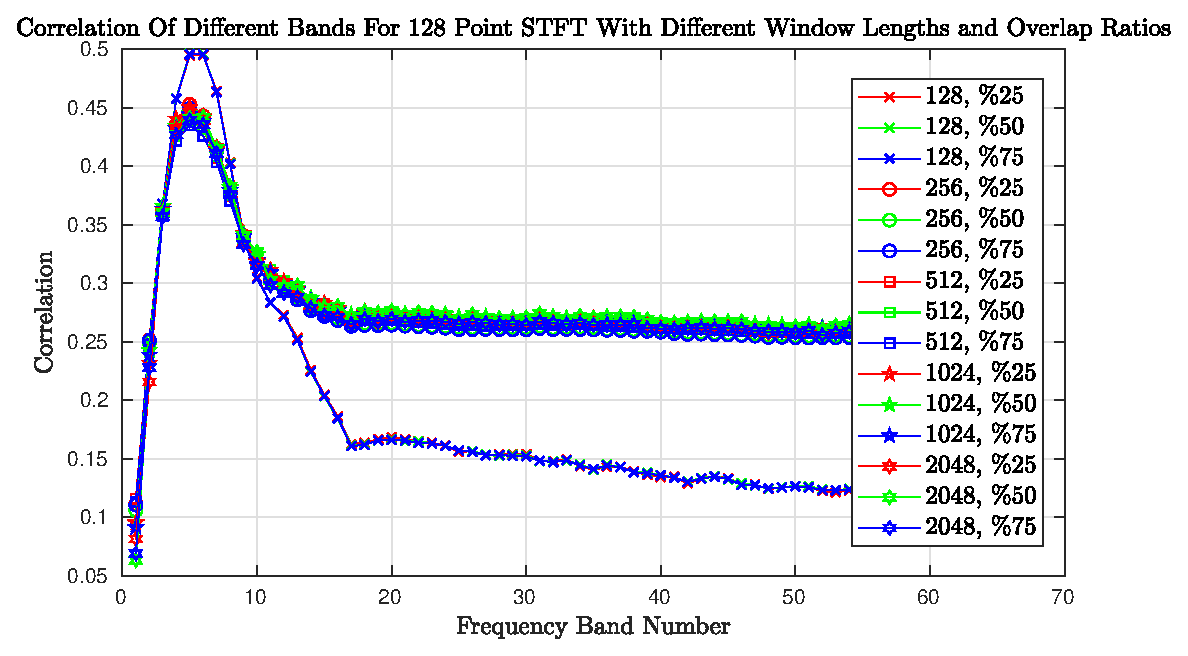
\includegraphics[width=\textwidth]{figures/corr_normal_for_stft_128.eps}
		\caption{Mean of correlations for each band for STFT method with 128 fft bins, window lengths and overlap ratios}
		\label{fig:airflow_stft_128}
	\end{center}
\end{figure}
\begin{figure}[h!]
	\begin{center}
		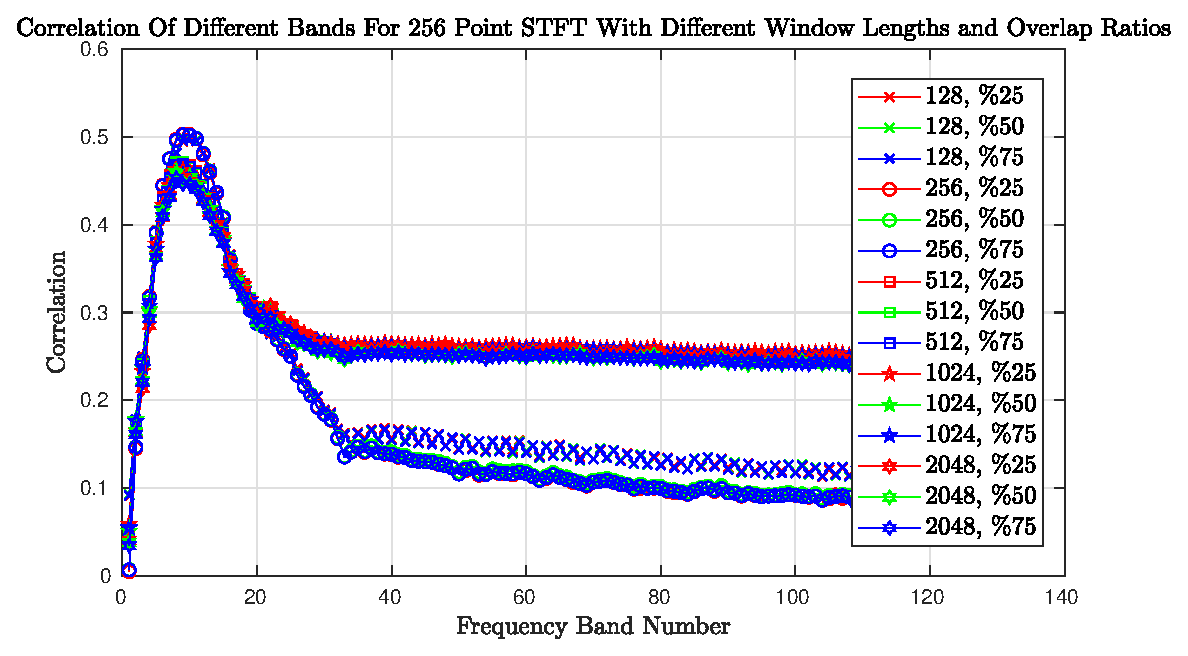
\includegraphics[width=\textwidth]{figures/corr_normal_for_stft_256.eps}
		\caption{Mean of correlations for each band for STFT method with 256 fft bins, window lengths and overlap ratios}
		\label{fig:airflow_stft_256}
	\end{center}
\end{figure}

\subsection{Unifying Estimations}
We run simulations with different number of vectors to be unified, where the vectors are outputs of univariate AR and STFT methods.
\begin{figure}[h!]
	\begin{center}
		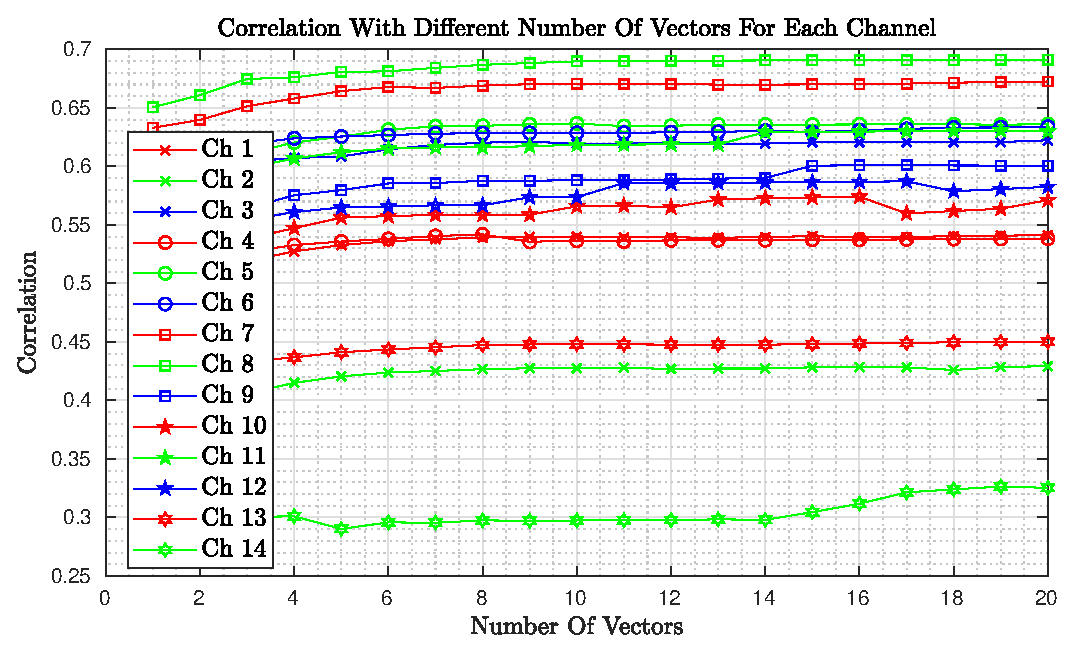
\includegraphics[width=\textwidth]{figures/corr_normal_unify.eps}
		\caption{Mean of correlations for each channel with different number of vectors unified}
		\label{fig:airflow_unify}
	\end{center}
\end{figure}
       

\subsection{Result}
\begin{table}[h!]
	\centering
	\begin{tabular}{|| c c c c ||} 
		\hline
		Channel & Univariate AR & Basis Functions & Kalman \\ [0.5ex] 
		\hline\hline
		1 & 0.6871 & 0.6862 & 0.6290 \\ 
		2 & 0.7440 & 0.7280 & 0.6802 \\
		3 & 0.6800 & 0.6699 & 0.6647 \\
		4 & 0.6310 & 0.6185 & 0.6536\\
		5 & 0.6153 & 0.6047 & 0.6649 \\
		6 & 0.5935 & 0.5963 & 0.6134 \\ 
		7 & 0.6031 & 0.6031 & 0.6328 \\ 
		8 & 0.5980 & 0.5885 & 0.6672 \\ 
		9 & 0.5761 & 0.5828 & 0.6351 \\ 
		10 & 0.5900 & 0.6009 & 0.6328 \\ 
		11 & 0.5681 & 0.5500 & 0.6197 \\ 
		12 & 0.5688 & 0.5719 & 0.6362 \\ 
		13 & 0.5733 & 0.5652 & 0.6127 \\ 
		14 & 0.5952 & 0.5916 & 0.5706 \\ 
		\hline
		\end{tabular}
		\caption{Correlation For Different Methods for All Channels}
		\label{table:1}
\end{table}
\chapter{AIRFLOW PHASE ESTIMATION}
\label{chp:airflow_phase_estimation}
We will present more than one methods to estimate the respiratory phases in this chapter. In one approach we will use the estimated airflow and in the other approach we will not use that, we directly use neural networks. In both methods we will use the estimation of breathing period.
\section{Period Estimation}
We assume that the period of breathing doesn't change abruptly and stay almost constant for each recording. In order to estimate the period we look at the autocorrelation function. For a periodic wave, the autocorrelation function is also periodic with the same period and there are peaks at the integer products of period. So, the period can be estimated by calculating the distances between the peaks. However, since the signal is noisy there are many local maxima, so instead of estimating the distance between peaks, we looked at the autocorrelation function of autocorrelation function of the signal that is being analyzed, and use the location of the maximum of local peaks in the part that is determined by minimum and maximum period. The equation for estimated period is given in \eqref{period_estimation}
\begin{equation}
T' = period_{min} + argmax(R_{R_{x}}[period_{min}:period_{max}])
\label{period_estimation}
\end{equation}
\begin{figure}
	\begin{center}
		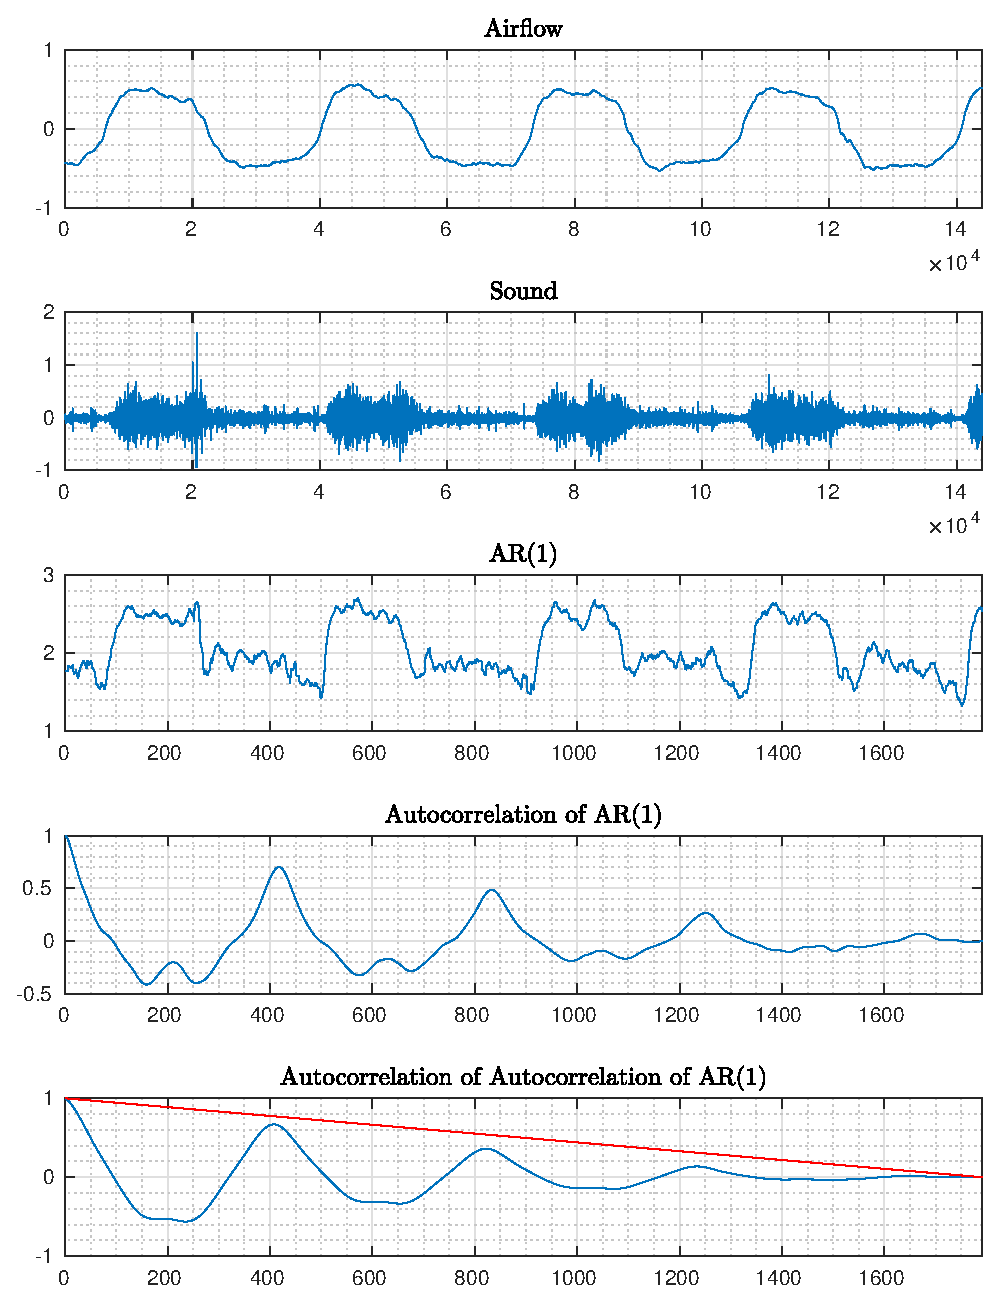
\includegraphics[width=\textwidth]{figures/find_period_ins_exp.eps}
		\caption{Visual Description Of Period Estimation}
		\label{fig:estimate_period}
	\end{center}
\end{figure}

\section{Phase Estimation With Neural Networks}
We try to use a neural network to decide the phase of a given signal segment. We decided to use the following features: AR coefficients, Shannon entropy estimate, percentile frequencies ($f_{25}$, $f_{50}$, $f_{75}$ and $f_{90}$) and the ratio between each of them, variance, spectral magnitude and kurtosis. These features change for each recording, bu the difference between inspiration and expiration doesn't change, so we used z-score before giving these features to neural network. A visual description of estimating the period is given in Figure \ref{fig:estimate_period}. We are looking at the ratio of blue function to the red line at the end.

\subsection{Description of Neural Networks} 
A neural network is a function with many inputs and a single output. Formulation and development of neural networks are inspired from biological nervous system. Input values of a neural network is processed by dozens of interconnected functions, and these functions are called "neuron"s. A neuron can be thought as a function with multiple outputs and a single output. A neuron's output is determined by the activation function \cite{neural-networks}.
\subsubsection{Neuron}
Mathematical expression of a neuron's activation function is given in \eqref{neuron_equation}. Here $\beta$ is the activation function. Activation function may be in several different forms. It is selected based on the application where the neural network is used and the distribution of input values. Activation functions are generally selected or constructed in a way that they are easily differentiable. Some of popular activation functions are given in  figure \ref{fig:activation_fncs}. 
\begin{equation} \label{neuron_equation}
y = \beta(\sum_{i=1}^{N}(w_ix_i))
\end{equation}
\begin{figure}[h] \label{neuron}
	\centering
\tikzstyle{inputNode}=[draw,circle,minimum size=10pt,inner sep=0pt]
\tikzstyle{stateTransition}=[->, thick]
\begin{tikzpicture}
\node[draw,circle,minimum size=25pt,inner sep=0pt] (x) at (0,0) {$\Sigma$};
\node[draw,circle,minimum size=25pt,inner sep=0pt] (y) at (2,0) {$\beta$};

\node[inputNode] (x0) at (-2, 1.5) {$\tiny x_0$};
\node[inputNode] (x1) at (-2, 0.75) {$\tiny x_1$};
\node[inputNode] (x2) at (-2, 0) {$\tiny x_2$};
\node[inputNode] (x3) at (-2, -0.75) {$\tiny x_3$};
\node[inputNode] (xn) at (-2, -1.75) {$\tiny x_n$};

\draw[stateTransition] (x0) to[out=0,in=120] node [midway, sloped, above=-2] {$w_0$} (x);
\draw[stateTransition] (x1) to[out=0,in=150] node [midway, sloped, above=-2] {$w_1$} (x);
\draw[stateTransition] (x2) to[out=0,in=180] node [midway, sloped, above=-2] {$w_2$} (x);
\draw[stateTransition] (x3) to[out=0,in=210] node [midway, sloped, above=-2] {$w_3$} (x);
\draw[stateTransition] (xn) to[out=0,in=240] node [midway, sloped, above=-2] {$w_n$} (x);
\node (dots) at (-2, -1.15) {$\vdots$};
\draw[stateTransition] (x) to[out=2,in=180] node [midway, above=-2] {$f$} (y);
\draw[stateTransition] (y) -- (3,0) node [right,right=-2] {$y$};;
\end{tikzpicture}
\caption{Diagram of A Neuron}
\end{figure}
\begin{figure}
	\begin{center}
		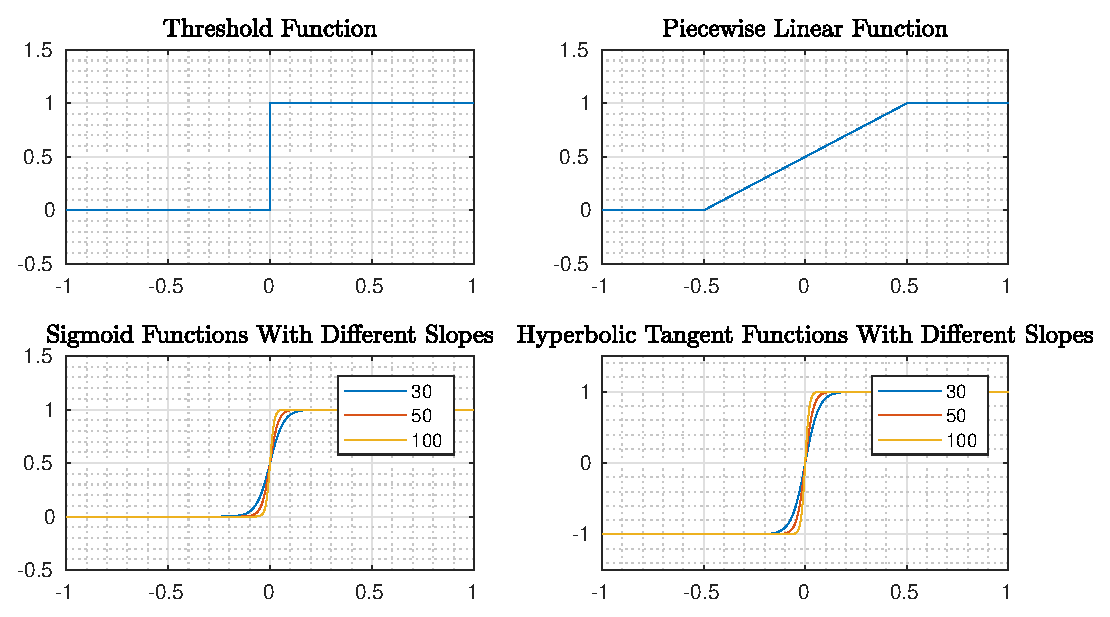
\includegraphics[width=\textwidth]{figures/several_activations.eps}
		\caption{Some Activation Functions}
		\label{fig:activation_fncs}
	\end{center}
\end{figure}
\subsubsection{Layers In Neural Networks}
There are three different layers in neural networks, input layer, output layer and hidden layers. Input and output layers are where the input values are received and output values are given out respectively. Hidden layers are where the information from input layer or previous hidden layer is processed. Hidden layers may have arbitrary number of neurons and there may be any number of hidden layers in a neural network.
\def\layersep{2.5cm}
\begin{figure}[h]
	\centering
	
\begin{tikzpicture}[shorten >=1pt,->,draw=black!50, node distance=\layersep]
\tikzstyle{every pin edge}=[<-,shorten <=1pt]
\tikzstyle{neuron}=[circle,fill=black!25,minimum size=17pt,inner sep=0pt]
\tikzstyle{input neuron}=[neuron];
\tikzstyle{output neuron}=[neuron];
\tikzstyle{hidden neuron}=[neuron];
\tikzstyle{annot} = [text width=4em, text centered]

% Draw the input layer nodes
\foreach \name / \y in {1,...,4}
% This is the same as writing \foreach \name / \y in {1/1,2/2,3/3,4/4}
\node[input neuron, pin=left:$x_\y$] (I-\name) at (0,-\y) {};

% Draw the hidden layer nodes
\foreach \name / \y in {1,...,5}
\path[yshift=0.5cm]
node[hidden neuron] (H-\name) at (\layersep,-\y cm) {};

% Draw the output layer node
\node[output neuron,pin={[pin edge={->}]right:Output}, right of=H-3] (O) {};

% Connect every node in the input layer with every node in the
% hidden layer.
\foreach \source in {1,...,4}
\foreach \dest in {1,...,5}
\path (I-\source) edge (H-\dest);

% Connect every node in the hidden layer with the output layer
\foreach \source in {1,...,5}
\path (H-\source) edge (O);

% Annotate the layers
\node[annot,above of=H-1, node distance=1cm] (hl) {Hidden layer};
\node[annot,left of=hl] {Input layer};
\node[annot,right of=hl] {Output layer};
\end{tikzpicture}
\caption{A Neural Network With One Hidden Layer}
\end{figure}

\subsubsection{Learning Process In Neural Networks}
Learning is the primary property of neural networks; it enables a neural network to improve its performance. \par 
The learning processes can be divided into three categories with respect to the learning paradigms. These categories are supervised, reinforcement and unsupervised learning. In supervised learning, the desired output is available so the error is known in the learning process. In reinforcement learning there is a performance measure which is being tried to be maximized. In unsupervised learning, neither desired output nor performance measure is available. We will use  supervised learning since the correct phases are known to us. \par
Learning methods can be divided into four sections, error-correction learning, memory based learning, Hebbian learning, competitive learning and Boltzmann learning. We will use error-correction learning and try to minimize the total error measure by adjusting the synaptic weights.
\subsection{Features}
In this section, we will look at the features that will be used in neural network approach. Each feature is found for all the sounds. However while looking at features, one can see that the patterns don't change however the range of values change. To overcome this issue each feature series from each sound gets normalized by  using z-score. Z-score is the measure which gives how much distance a random sample has to its source mean. The formula for z-score is given in \eqref{eq:z-score}
\begin{equation}\label{eq:z-score}
z_i = \frac{x_i - \hat{\mu}_X}{\hat{\sigma}_X}
\end{equation} \par
We also used the Kullback-Leibler (KL) divergence to quantify how much the distributions for inspiration and expiration differ from each other for each feature. KL-divergence is a definition from information theory and it gives a distance between probability distributions. The formula for KL-divergence is given in \eqref{eq:kl-divergence} \cite{info-theory}.
\begin{equation}\label{eq:kl-divergence}
D_{KL}(p(x)||q(x)) = \sum_{x \in X}p(x)\log\frac{q(x)}{p(x)}
\end{equation} 
\subsubsection{AR Coefficients}
When we modeled the respiratory sounds as AR processes and solve for the AR coefficients, we saw that estimated AR coefficients are behaving differently for inspiration and expiration. To give an example, for the case of first AR coefficient it seems as the coefficients are attenuated for expiration phases. So we decided to use  AR coefficients as a feature to the neural network. A detailed explanation about AR models and methods to estimate AR coefficients is given in Section \ref{chp:airflow_curve_estimation}. \\ Distributions of AR coefficients during inspiration and expiration for third channel is given in Figure \ref{fig:arall_ins_exp}
\begin{figure}[h!]
	\begin{center}
		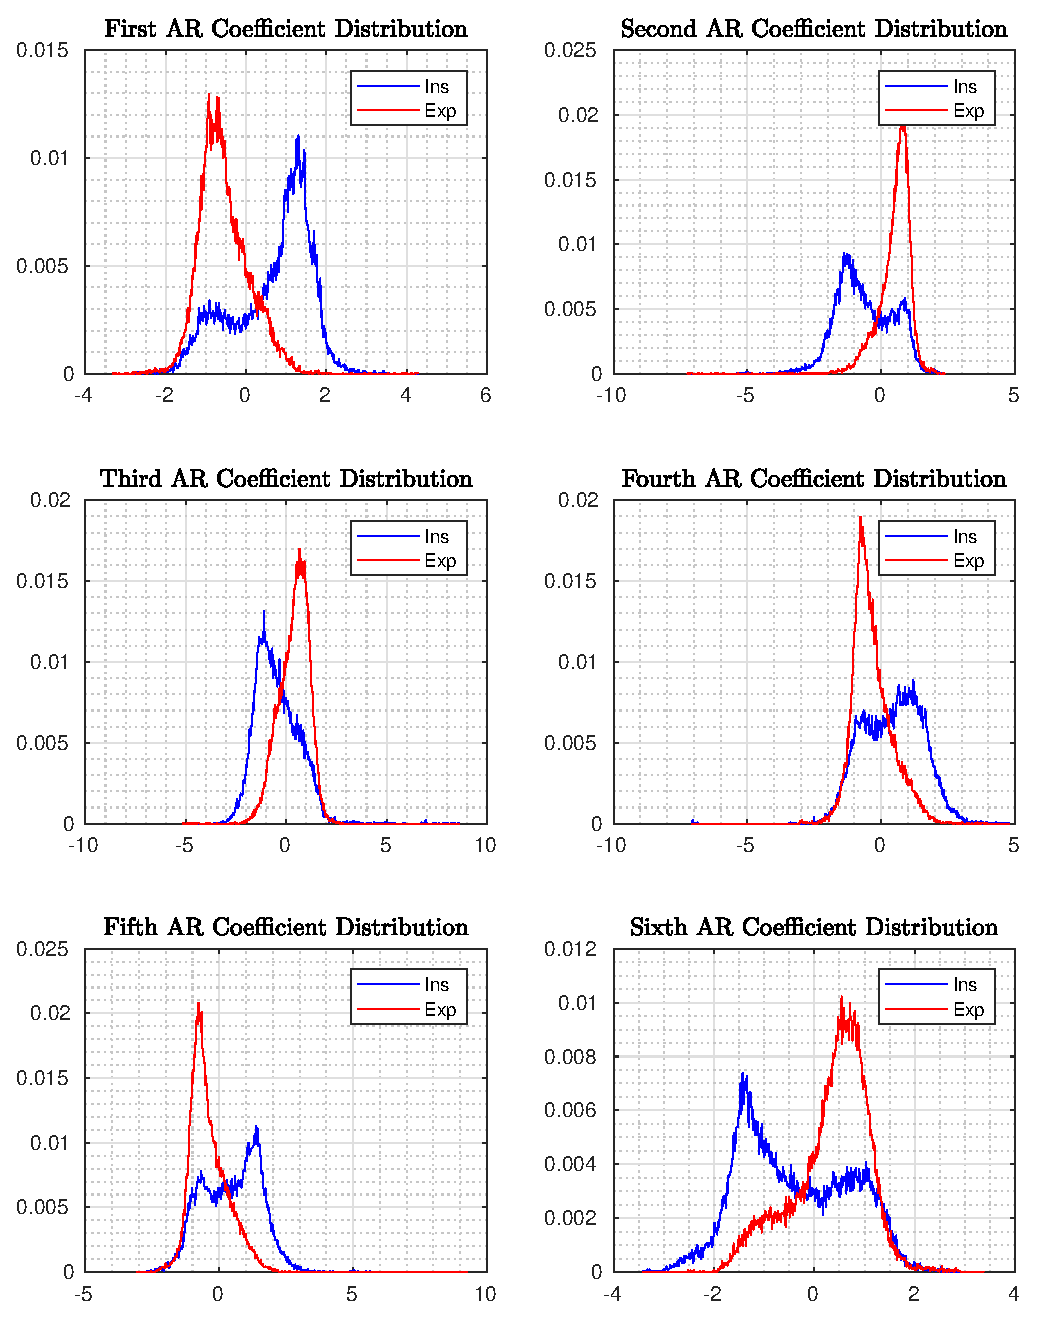
\includegraphics[width=\textwidth]{figures/arall_ins_exp.eps}
		\caption{Distribution of AR Coefficients For Inspiration and Expiration}
		\label{fig:arall_ins_exp}
	\end{center}
\end{figure}
\subsubsection{Shannon Entropy Estimate}
Entropy is a measure which gives information about the complexity of the samples collected. As the randomness of the samples increases entropy increases too. The formula to calculate entropy is given in \eqref{eq:entropy} \cite{info-theory}.  In general we have a wider range for signal values in inspiration, so we expect entropy to be greater for the segments belonging to inspiration. \\ Distributions of Shannon's entropy estimates during inspiration and expiration for third channel is given in Figure \ref{fig:entropy_ins_exp}
\begin{equation}\label{eq:entropy}
	H(X) = - \sum_{x \in X}p(x)\log(x)
\end{equation}
\begin{figure}
	\begin{center}
		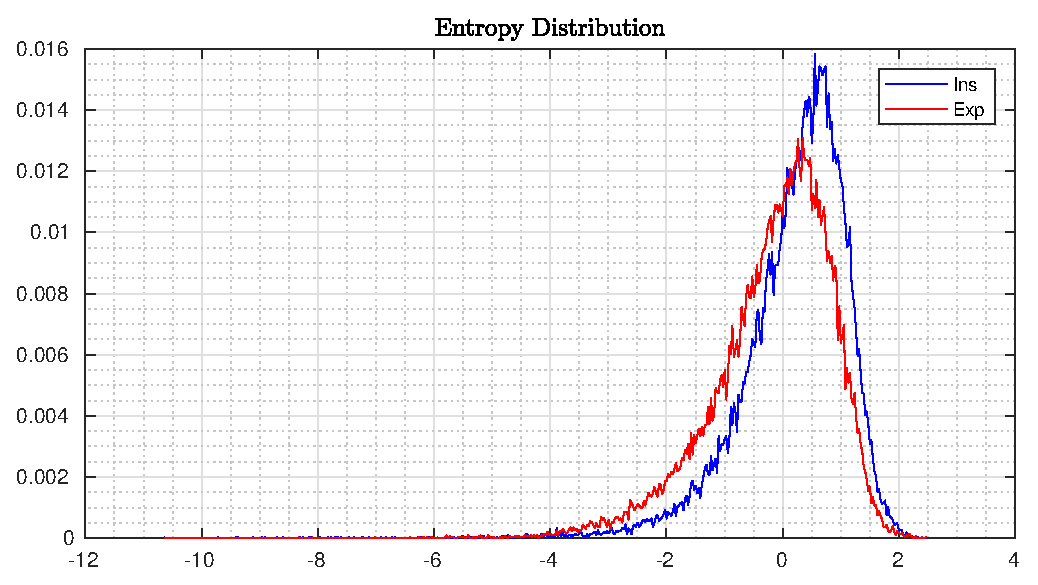
\includegraphics[width=\textwidth]{figures/entropy_ins_exp.eps}
		\caption{Distribution of Shannon Entropy Estimate For Inspiration and Expiration}
		\label{fig:entropy_ins_exp}
	\end{center}
\end{figure} 
\subsubsection{Percentile Frequencies}
A percentile frequency is defined together with the percent. It is the frequency until which the cumulative sum of power spectral density is equal to the defined percent of total power. In order to calculate them, we first estimate the power spectral density according to the formula in Percentile frequencies and their relations are measures which are widely used in respiratory signal analysis \cite{sergul, comparison-ar-based}. Since the expiration and inspiration phases have different time-frequency content, percentile frequencies may be used as input to classifier neural network. Definition of a percentile frequency is given in \eqref{percentf} \\ Distributions of percentile frequencies and their ratios between each other during inspiration and expiration for third channel is given in Figure \ref{fig:percent_ins_exp}.
\begin{align}
	X(f) = \int_{-\infty}^{\infty}x(t)e^{-2{\i}ft\pi}dt \label{ft} \\
	P_{XX}(f) = X(f)^2 \label{psd}\\
	f_{y} = \underset{x}\argmin \frac{\int_{0}^{x} P_{XX}(f) df}{\int_{0}^{\infty} P_{XX}(f) df}   > \frac{y}{100} \label{percentf}
\end{align}
\begin{figure}
	\begin{center}
		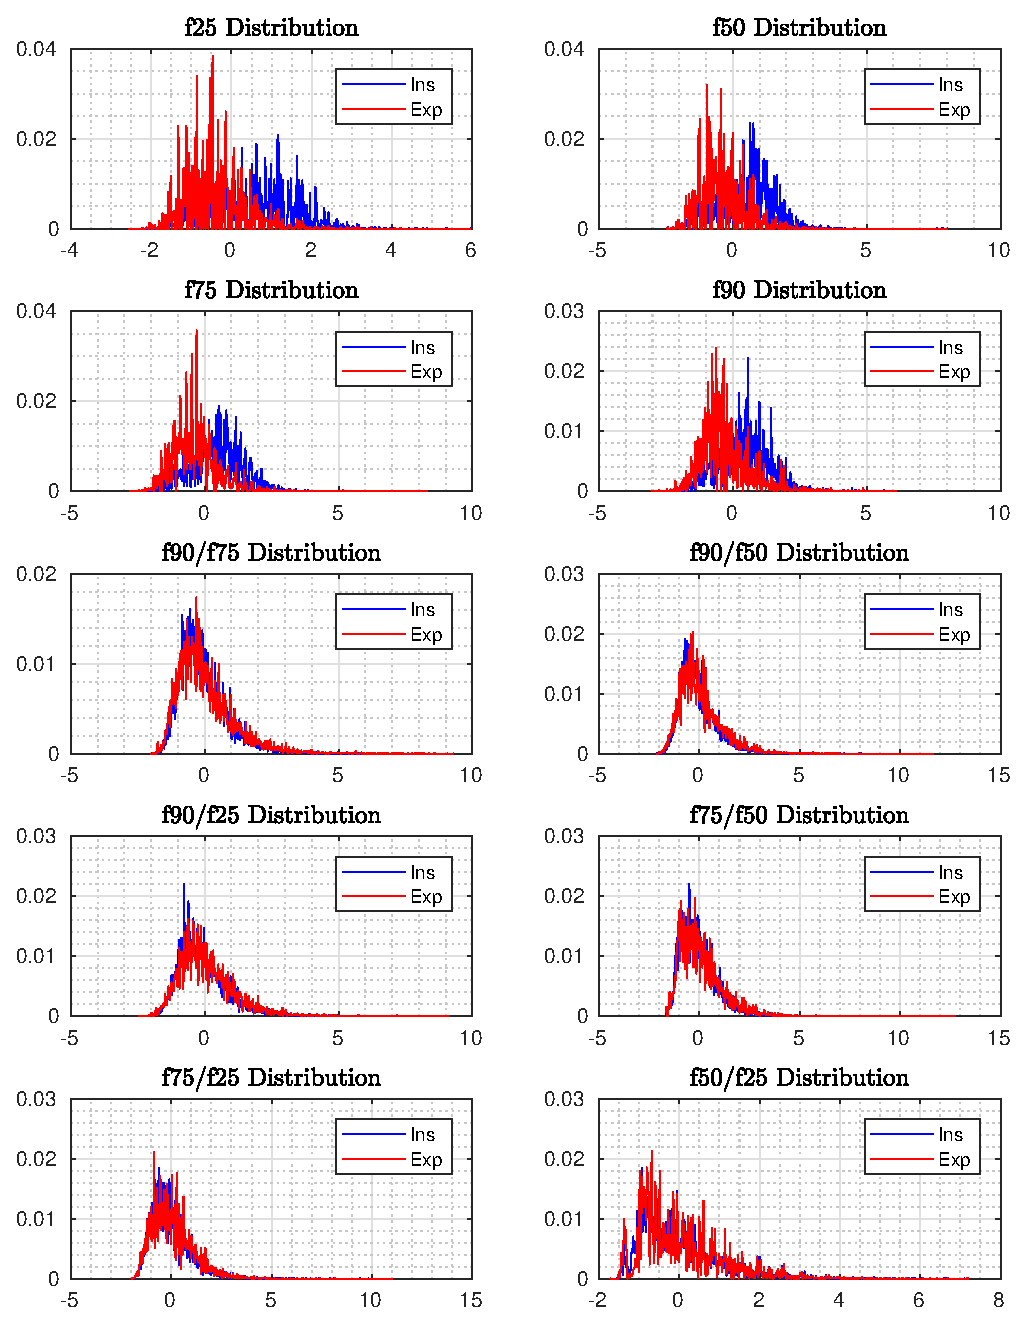
\includegraphics[width=\textwidth]{figures/percent_ins_exp.eps}
		\caption{Distribution of Percentile Frequency Measures For Inspiration and Expiration}
		\label{fig:percent_ins_exp}
	\end{center}
\end{figure}
\subsubsection{Variance}
Variance corresponds to power and observations show that power for different respiratory phases differs. So we decided to use variance as a supportive feature. Sample variance is calculated as in \eqref{sample_variance}. \\ Distributions of variance of windows during inspiration and expiration for third channel is given in Figure \ref{fig:percent_ins_exp}.
\begin{align}
	\hat{\mu}_{X} = \frac{\sum_{x \in X}x}{|X|} \label{sample_mean} \\
	\hat{\sigma}_{X}^2 = \frac{\sum_{x \in X}(x-\hat{\mu}_X)^2}{|X|-1}\label{sample_variance}
\end{align}
\begin{figure}
	\begin{center}
		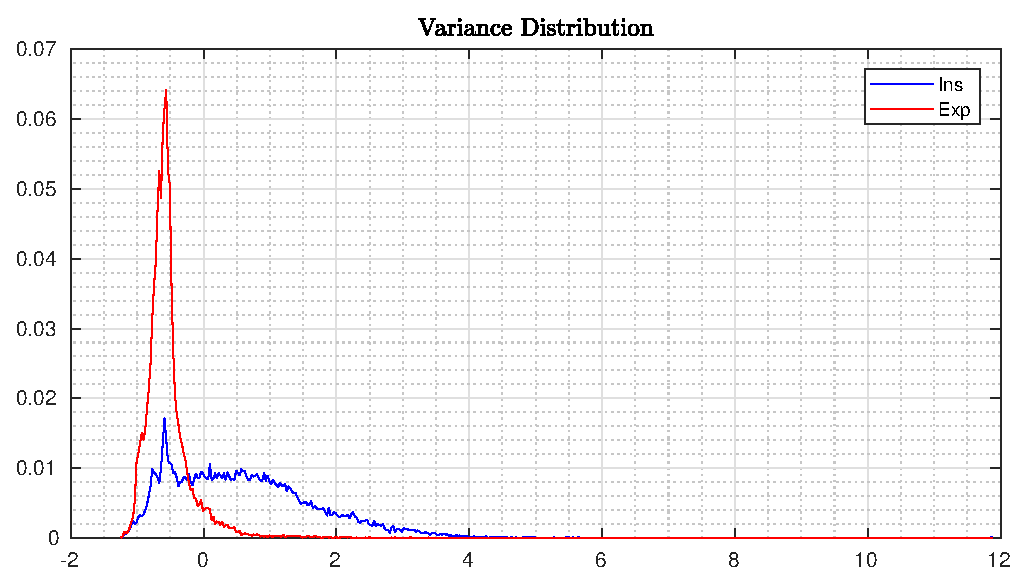
\includegraphics[width=\textwidth]{figures/variance_ins_exp.eps}
		\caption{Distribution of Variance For Inspiration and Expiration}
		\label{fig:variance_ins_exp}
	\end{center}
\end{figure}
\subsubsection{Spectral Magnitude}
The magnitudes of several frequency bands are calculated for each segment using FFT. We calculated the spectral band's magnitude by taking FFT of windows after multiplying them a Hamming window for smoothing. We used 128 points FFT and each band represents a band of 75 Hz. We used the following bands' magnitudes: \{150 Hz-225 Hz, 225 Hz-300 Hz, 300 Hz-375 Hz, 375 Hz-450 Hz\}. \\ Distributions of spectral magnitudes of windows during inspiration and expiration for third channel is given in Figure \ref{fig:spectral_ins_exp}. 
\begin{figure}
	\begin{center}
		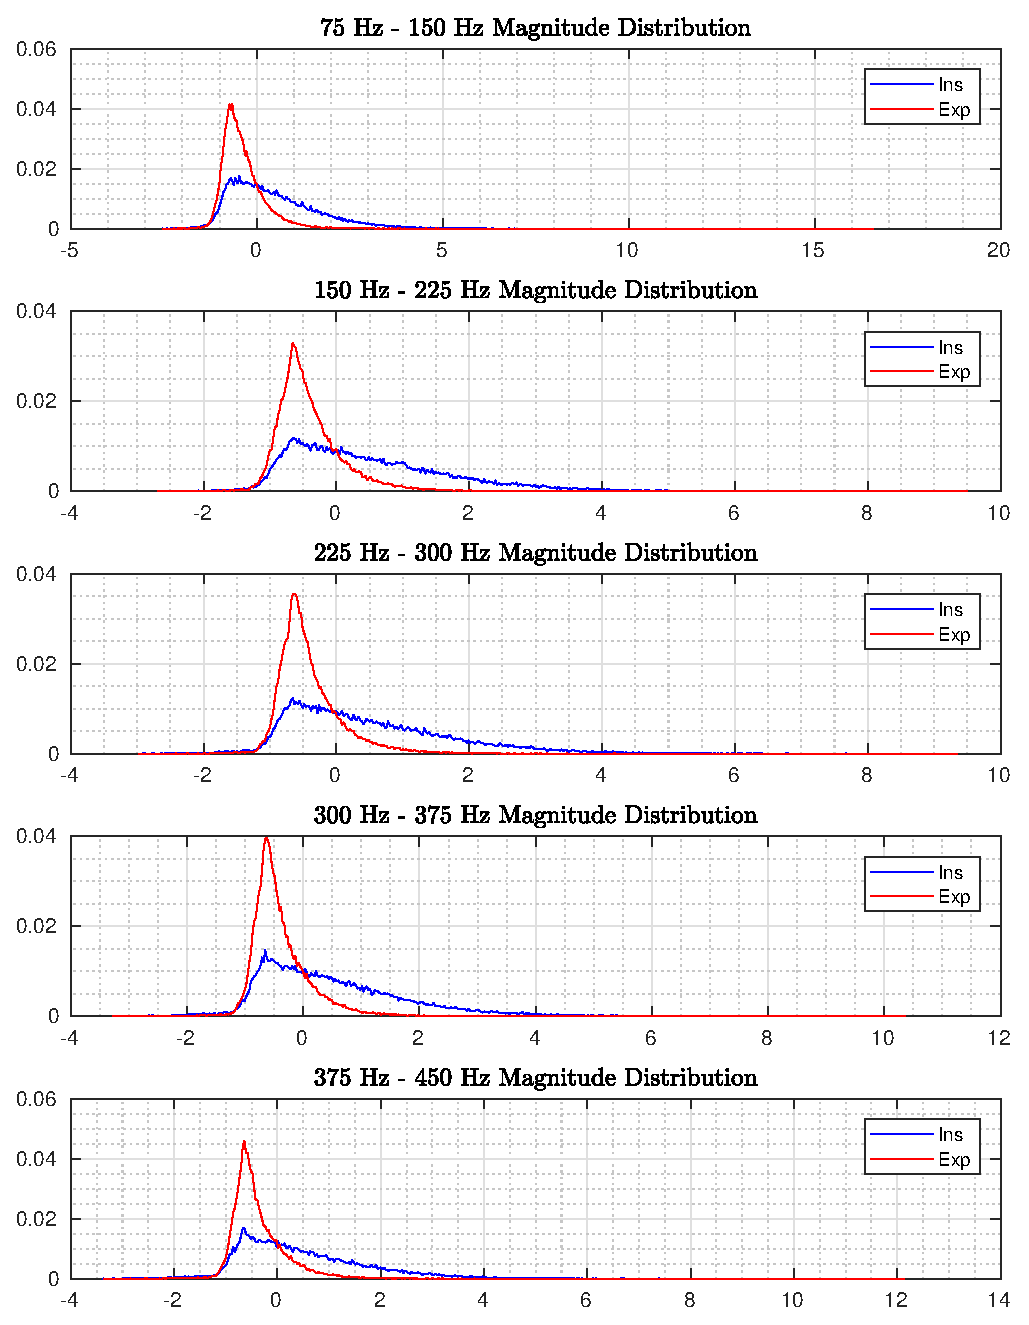
\includegraphics[width=\textwidth]{figures/spectral_ins_exp.eps}
		\caption{Distribution of Spectral Magnitudes For Inspiration and Expiration}
		\label{fig:spectral_ins_exp}
	\end{center}
\end{figure}
\subsubsection{Kurtosis}
Kurtosis is the ratio of the fourth moment to square of second moment. It is a statistical feature which have been used in respiratory signal analysis. Formula for kurtosis is given in \eqref{eq:kurtosis}\\ Distributions of kurtosis of windows during inspiration and expiration for third channel is given in Figure \ref{fig:kurtosis_ins_exp}. 
\begin{equation}\label{eq:kurtosis}
K = |X|\frac{\sum_{x \in X}(x-\hat{\mu}_X)^4}{(\sum_{x \in X}(x-\hat{\mu}_X)^2)^2}
\end{equation}
\begin{figure}
	\begin{center}
		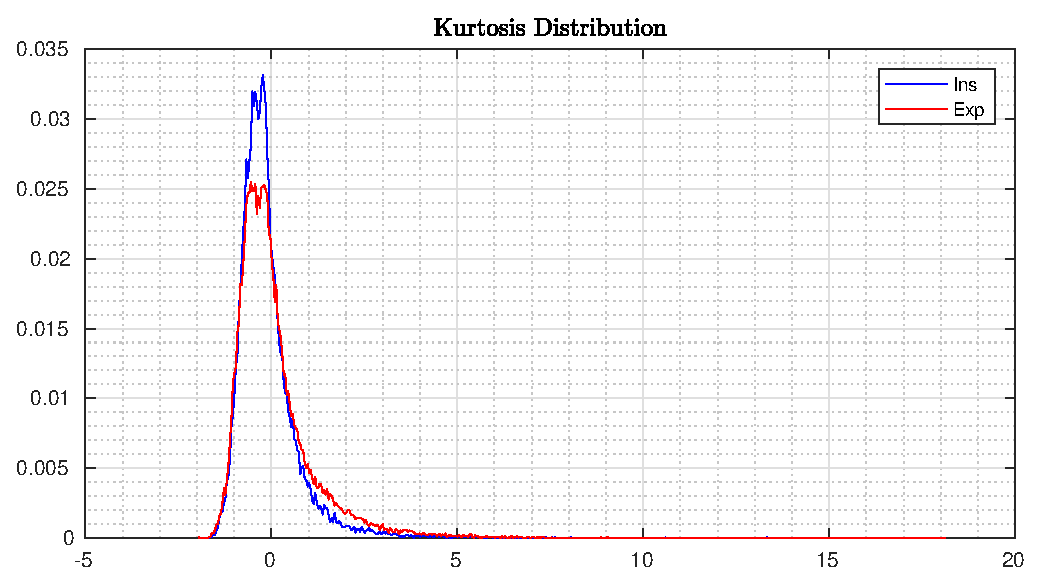
\includegraphics[width=\textwidth]{figures/kurtosis_ins_exp.eps}
		\caption{Distribution of Kurtosis For Inspiration and Expiration}
		\label{fig:kurtosis_ins_exp}
	\end{center}
\end{figure} \par 
The average KL-divergence for features is given in figure \ref{fig:kl_divergence}. The feature indices are consistent with the order features are explained above.
\begin{figure}
	\begin{center}
		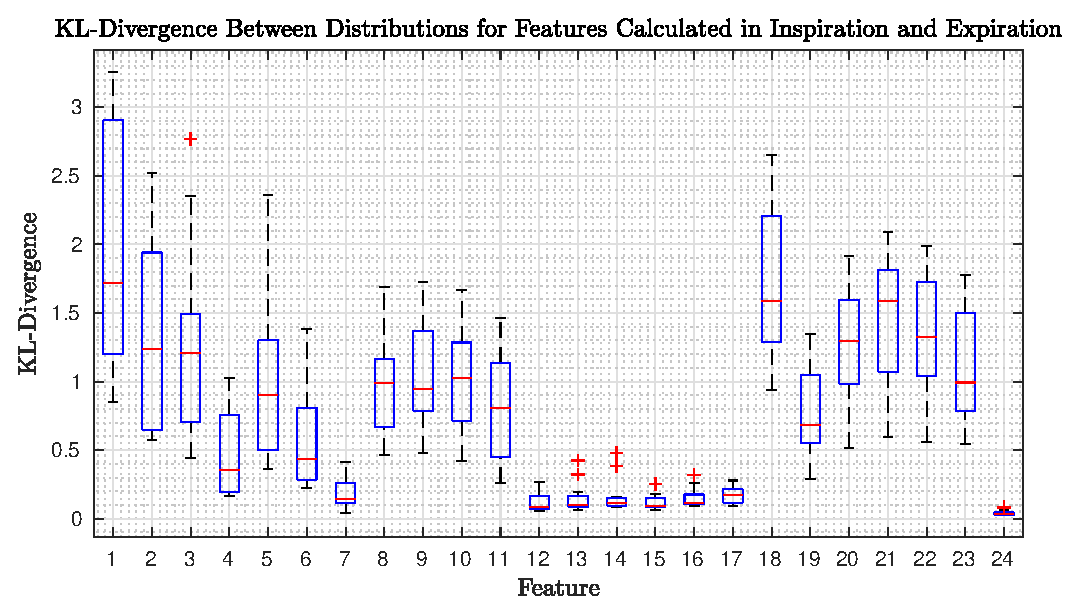
\includegraphics[width=\textwidth]{figures/kl_divergence.eps}
		\caption{KL-Divergence Between Distributions for Features Calculated in Inspiration and Expiration}
		\label{fig:kl_divergence}
	\end{center}
\end{figure} 
\subsection{Denoisining The Output of Neural Network}
The output of neural network is not very good in terms of estimating the phase correctly and it is alternating too much even in short durations. In order to overcome this issue, a filtering was needed. Linear filters don't perform well since they show many discontiunity, so we decided to use a filter that counts the contiunity into account and since we had estimated the period earlier, we tried to use that for filtering purposes. Then we created a periodic square wave with the period equal to the the estimated period and $50\%$ duty cycle. We calculated the cross correlation between this square wave and the output of neural network. This shows us the required amount of shift that is needed for the square wave to fit on to the phase of airflow. We must note that, here we assume that the airflow is periodic and its duty cycle is $50\%$. 
\section{Phase Estimation With Estimated Airflow Curve}
We try to estimate the airflow phase curve using the estimated airflow curves. In order to do that, we used the estimation which has the most correlation with the absolute airflow curve, so we used the first AR coefficient of consecutive and overlapping windows. It is reported that the onsets can be found by looking at local minima of estimated absolute airflow curve. In our case, local minima analysis only didn't solve the problem and we developed some heuristic algorithms based on our observations.
\subsection{Prefiltering}
We try to locate the local minima, but because of the noisy nature of estimated airflow, there are many false minima. Then we applied a median and moving average filter. We chose to use a median filter to filter out the spikes and a moving average filter to smooth the signal. Describing formulae for median and moving average filters with $2K+1$ taps are given in \eqref{eq:median_filter} and \eqref{eq:moving_average}.
\begin{equation}
	y_i = med(x_{\max(0,{i-K})}, x_{\max(0,{i-K+1})}, ... x_i, ..., x_{\min(L,{i+K-1})}, x_{\min(L,{i+K})})
	\label{eq:median_filter}
\end{equation}
\begin{equation}
y_i = \frac{\sum_{j=\max(0, i-K)}^{\min(L, i+K)}x_j}{\min(L, i+K) - \max(0, i-K) + 1}
\label{eq:moving_average}
\end{equation}
\paragraph{}A figure showing unfiltered and filtered signal is given in Figure \ref{fig:prefiltering}
\begin{figure}[h!]
	\begin{center}
		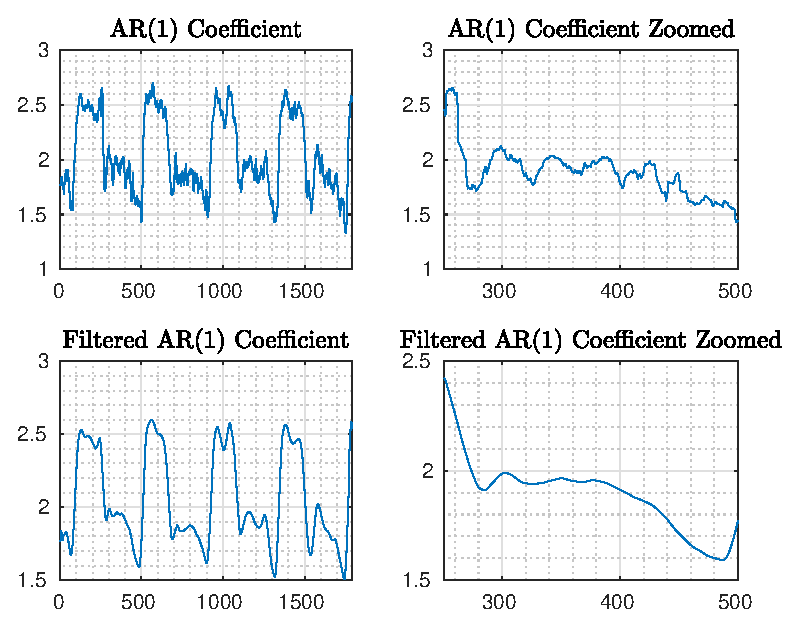
\includegraphics[width=\textwidth]{figures/prefiltering.eps}
		\caption{Filtering The Flow Estimate}
		\label{fig:prefiltering}
	\end{center}
\end{figure}
\subsection{Local Minima Extraction}
The number of local minima is decreased by filtering, however, it is still too much to process. So, we decided to add a heuristic algorithm to selection algorithm of local minima. We decided to use two types of local minimum, one type, let's call it $type$-1, is mostly seen in transition from expiration to inspiration and the other, $type$-2, is mostly seen in transition from inspiration to expiration. We don't expect any minima in the right neighborhood of $type$-1 minimum and in the left neighborhood of $type$-2 minimum for a certain amount of distance. 
The examples to $type$-1 and $type$-2 minima is shown in figure \ref{fig:minima}.
\begin{figure}
	\begin{center}
		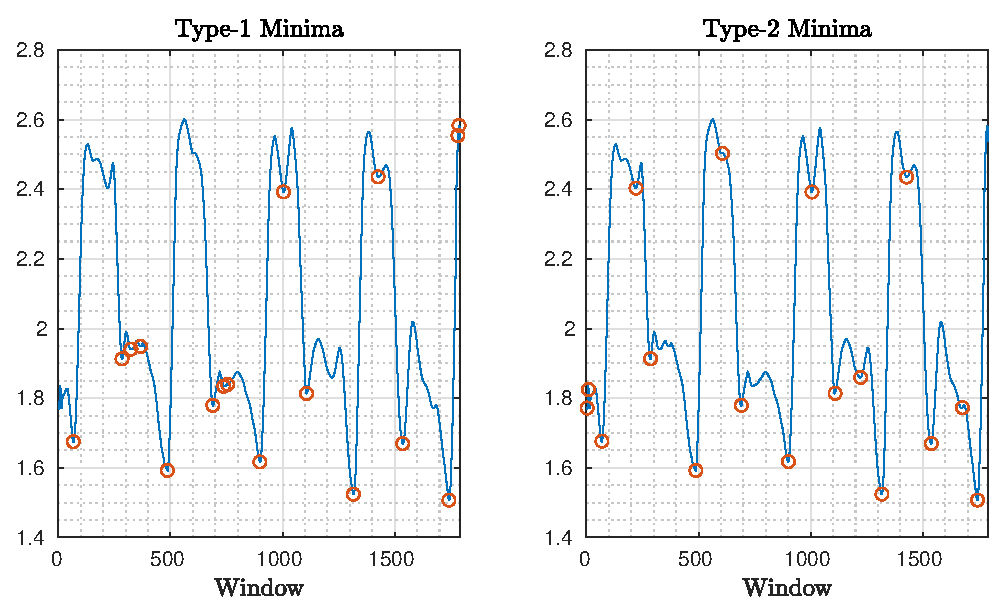
\includegraphics[width=\textwidth]{figures/minima.eps}
		\caption{Type-1 and Type-2 Minima}
		\label{fig:minima}
	\end{center}
\end{figure}
\subsection{Selection of Transition Points}
We use the period estimation and local minima together to decide on the location of transition points. While all the local minima are candidate transition points, we assume that the distribution of the distances between consecutive transitions from inspiration to expiration and expiration to inspiration have a distribution with a small variance and a mean which is equal to the period estimation. So, firstly, we decide on the number of transitions in each direction. Then we list all the subsets of local minima which has the number of transition elements. Finally we calculate the likelihoods of each subset according to \eqref{eq:likelihood} and select the one which has most. After selecting the first transition points set, in order to decide on the set belonging to the other transition type, we also look at the distance to the set of first transition type. In this method we don't assume any value for the duty cycle. An example of change point estimation is given in \ref{fig:transition}.
\begin{equation}
	L(\vec{d}) = \frac{\exp((\vec{d}-T')^T(\vec{d}-T')/\sigma^2)}{\sigma}
	\label{eq:likelihood} 
\end{equation}
\begin{figure}[h!]
	\begin{center}
		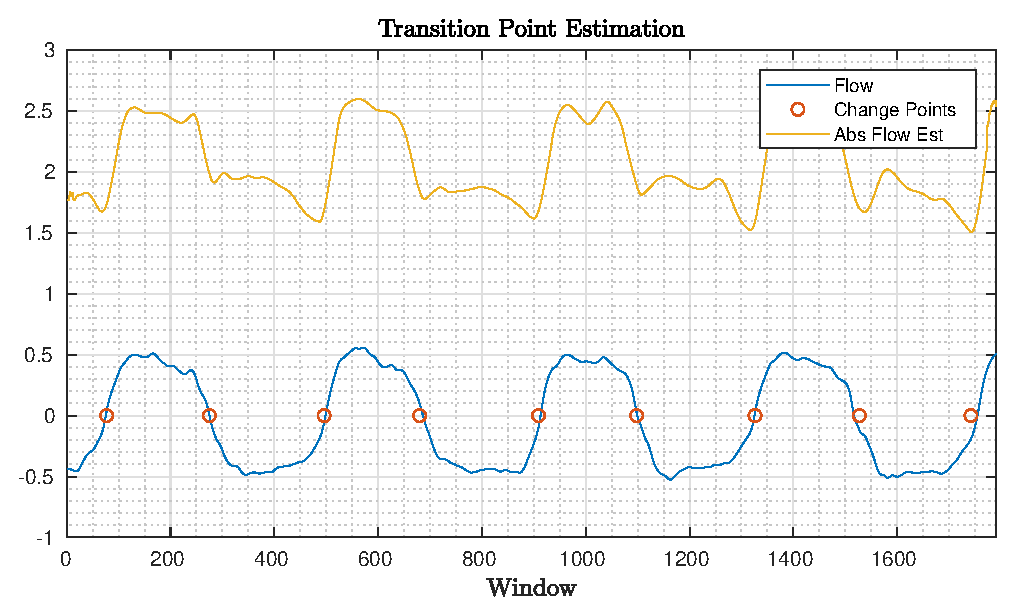
\includegraphics[width=\textwidth]{figures/transition.eps}
		\caption{Transition Point Estimation}
		\label{fig:transition}
	\end{center}
\end{figure}
\subsection{Estimating The Phases Given Transition Points}
We estimate the phases of segments after deciding on transition points by using the first AR coefficient of segments divided by the transitions points. We create two group and each group includes nonconsecutive segments. We then calculate the AR coefficients for each segment, and we label the group with a greater average AR coefficient as inspiration. This method works with a success rate of 96\%.
\section{Experiments \& Results}
\subsection{Neural Networks}
Matlab's neural network toolbox is used in training process. We selected the performance function to be cross-entropy since it is a standard \cite and training function to be scaled conjugate gradient. 
We used neural networks with different number of hidden neurons and the correlation of neural network's output and phase is not changing significantly with the number of hidden neurons. This experiment is done on third channel of 10 subjects. The boxplot showing results for different number of hidden neurons is given in figure \ref{fig:hidden}. So we decided to use 20 neurons.
\begin{figure}[h!]
	\begin{center}
		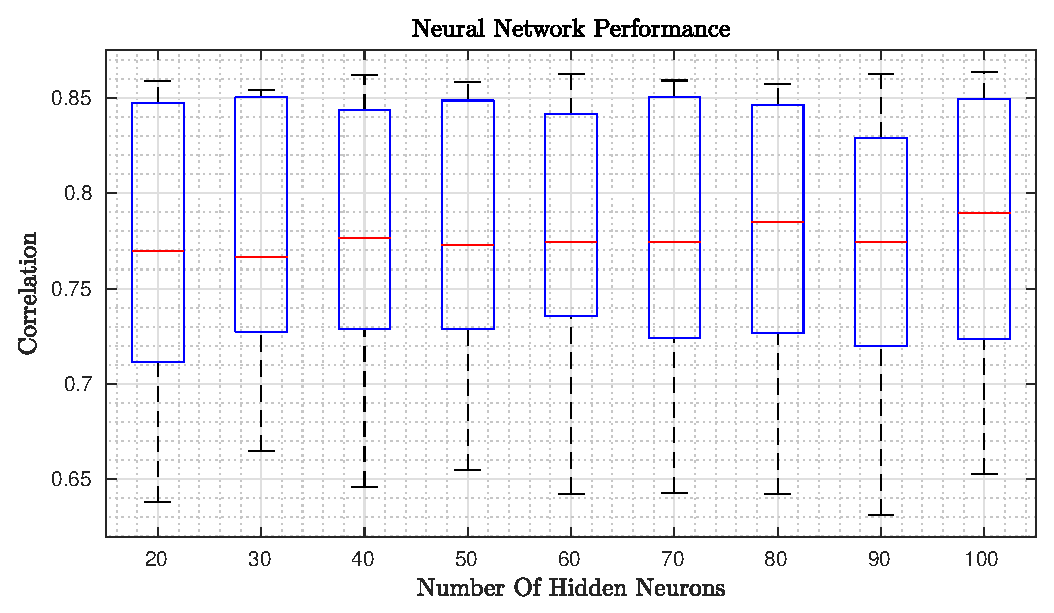
\includegraphics[width=\textwidth]{figures/hidden.eps}
		\caption{Performance of Neural Network vs Number of Hidden Neurons}
		\label{fig:hidden}
	\end{center}
\end{figure}
We measured the performance of neural networks by using correlation measure. The boxplot of correlation between neural network's output and the phase plot is given in \ref{fig:neur_net_corr}. We then corrected the output of neural networks by using the period information, and the result is shown in \ref{fig:neur_net_corr_corrected}.
\paragraph{} In addition to correlation measure we also measured the deviation of detected transition points from real transition points. We introduced a deadband which is equal to 5\% of peak-to-peak voltage around zero before calculating the true transition points.
\begin{table}[h!]
	\centering
	\begin{tabular}{|| c c c c c c c c c c c c c c ||} 
		\hline
		Channel & 1 & 2 & 3 & 4 & 5 & 6 & 7 & 8 & 9 & 10 & 11 & 12 & Average \\ [0.5ex] 
		\hline\hline
		Ins to Exp & 74 & 183 & 76 & 87 & 77 & 74 & 80 & 71 & 146 & 115 & 86 & 82 & 96.8\\ 
		Exp to Ins & 64 & 150 & 66 & 77 & 63 & 67 & 62 & 65 & 126 & 123 & 68 & 65 & 83.2\\
		\hline
	\end{tabular}
	\caption{Deviation From True Transitions in Milliseconds}
	\label{transition_deviation_neural}
\end{table}
\begin{figure}
	\begin{center}
		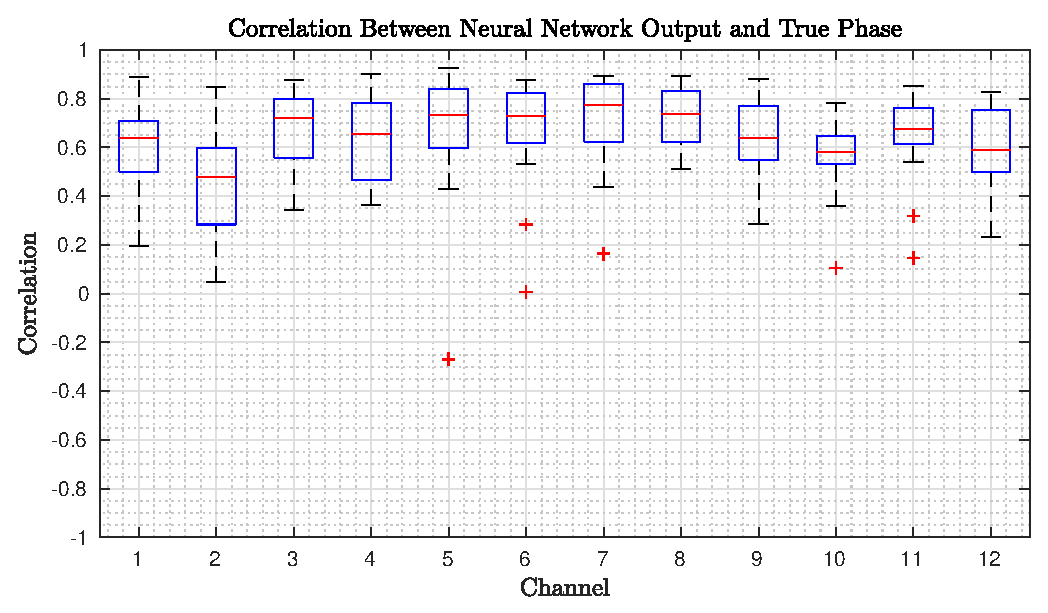
\includegraphics[width=\textwidth]{figures/neur_net_corr.eps}
		\caption{Performance of Neural Network vs Channels}
		\label{fig:neur_net_corr}
	\end{center}
\end{figure}

\begin{figure}
	\begin{center}
		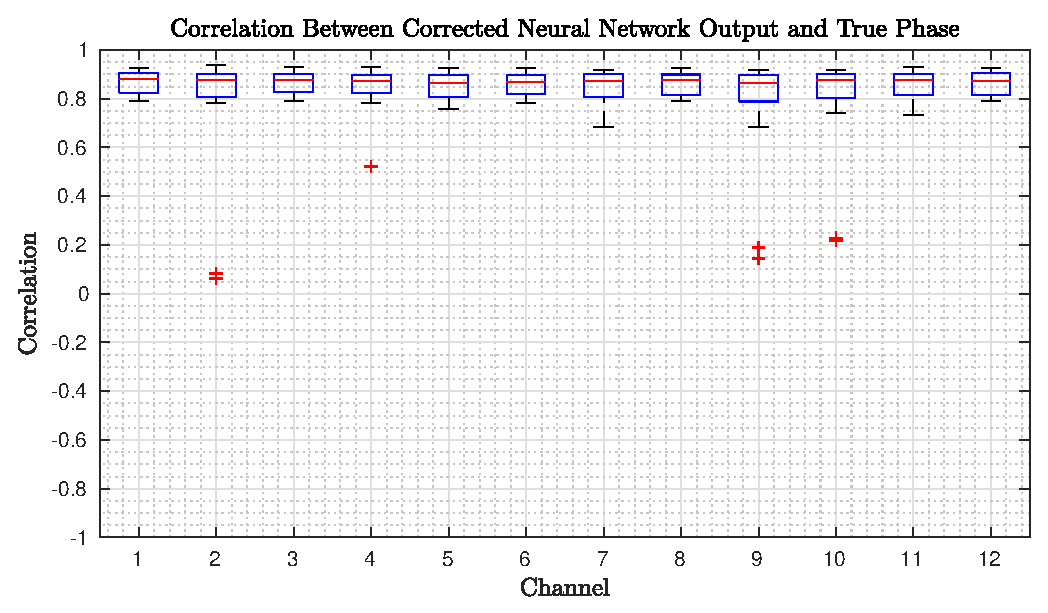
\includegraphics[width=\textwidth]{figures/neur_net_corr_corrected.eps}
		\caption{Performance of Neural Network vs Channels After Correction}
		\label{fig:neur_net_corr_corrected}
	\end{center}
\end{figure}

\subsection{Transition Points Detection Based On Local Minima}
We used first AR coefficient and period information to estimate transition points and calculated the first AR coefficient of the segments between transition points to decide on phase. The correlation between esimated and true flow phase is given in figure \ref{fig:local_minima_phase} and the deviation from true transitions is given in table \ref{transition_deviation_minima}.
\begin{table}[h!]
	\centering
	\begin{tabular}{|| c c c c c c c c c c c c c c ||} 
		\hline
		Channel & 1 & 2 & 3 & 4 & 5 & 6 & 7 & 8 & 9 & 10 & 11 & 12 & Average \\ [0.5ex] 
		\hline\hline
		Ins to Exp & 112 & 121 & 130 & 110 & 96 & 117 & 159 & 102 & 88 & 176 & 110 & 118 & 119.76\\ 
		Exp to Ins & 106 & 186 & 94 & 198 & 113 & 117 & 157 & 149 & 104 & 143 & 131 & 131 & 130.73\\
		\hline
	\end{tabular}
	\caption{Deviation From True Transitions in Milliseconds}
	\label{transition_deviation_minima}
\end{table}

\begin{figure}
	\begin{center}
		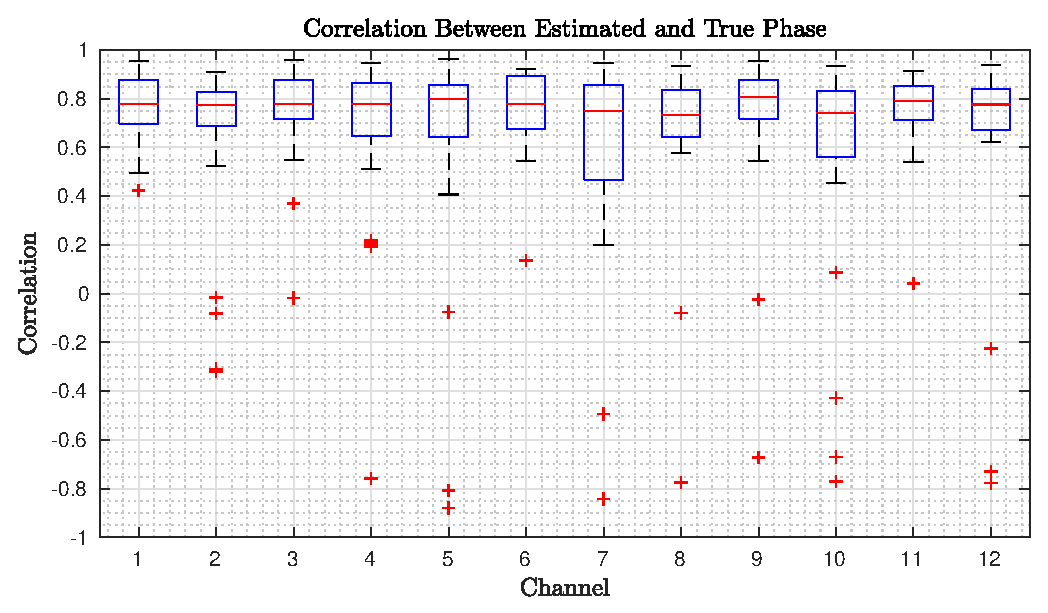
\includegraphics[width=\textwidth]{figures/local_minima_phase.eps}
		\caption{Performance of Phase Estimation Based On Local Minima}
		\label{fig:local_minima_phase}
	\end{center}
\end{figure}

\chapter{CONCLUSION}
\label{chp:conclusion}
In this thesis, we suggested and tested methods, some of which were already suggested, to estimate the curve and phase of the airflow over the mouth by using the sounds recorded on chest wall. The airflow and its phase have diagnostic value, so the accurate estimation of them may increase pulmonary disease detector's performance in case there is no airflow measurement.
\par In chapter \ref{chp:airflow_curve_estimation}, we tested the TVAR modeling of respiratory sounds approach after we gave description of AR and TVAR processes. The method in (Koray) uses the basis functions to estimate the TVAR coefficients, we also implemented the windowing based and Kalman filter approaches and measured the performance by looking at the correlation coefficient between estimation and absolute value of airflow. From the results, it can be said that, all three approaches have similar performance. Later, we tested the correlation of magnitudes of different frequency bands with the airflow itself. Lastly, we introduced the Wiener filter approach to unify different estimations of airflow.
\par In chapter \ref{chp:airflow_phase_estimation}, we first gave a method to estimate the period of breathing from the estimation of airflow, which was the first AR coefficient. Then, we worked with a neural network for classification of inspiration and expiration. We presented the histograms of features (AR, Time-Frequency, Percentile Frequencies, Variance, Entropy and Kurtosis) from inspiration and expiration parts. We then presented a method to denoise the output of neural networks by using the period information and assuming a 50\% duty cycle. We also try to estimate the transition points by using the absolute airflow estimation and the period information. 
\par To sum up, the relation between respiratory sounds, their features and the airflow is explored throughout this thesis. It can be concluded that, the phase information can be extracted from respiratory sounds with a good performance by using the techniques in chapter \ref{chp:airflow_phase_estimation} and the airflow curve can be estimated with the techniques in chapter \ref{chp:airflow_curve_estimation} but with a less performance compared to phase estimation.
\bibliographystyle{styles/fbe_tez_v11}
\bibliography{references}

\end{document}